\documentclass[10pt,conference]{IEEEtran}
\IEEEoverridecommandlockouts
% The preceding line is only needed to identify funding in the first footnote. If that is unneeded, please comment it out.
\usepackage{cite}
\usepackage{amsmath,amssymb,amsfonts}
\usepackage{algorithmic}
\usepackage{algorithm}
\usepackage{graphicx}
\usepackage{textcomp}
\usepackage{xcolor}
\def\BibTeX{{\rm B\kern-.05em{\sc i\kern-.025em b}\kern-.08em
    T\kern-.1667em\lower.7ex\hbox{E}\kern-.125emX}}
\begin{document}

\title{COLAB: A Collaborative Multi-factor Scheduler for Asymmetric Multicore Processors
%\thanks{Identify applicable funding agency here. If none, delete this.}
}

%\author{\IEEEauthorblockN{double-blind review\textsuperscript{} }
%\IEEEauthorblockA{\textit{dept. name of organization (of Aff.)} \\
%\textit{name of organization (of Aff.)}\\
%City, Country \\
%email address}
%\and
%}

\maketitle
%%%%%%%%%%%---SETME-----%%%%%%%%%%%%%
%\title{COLAB: A Collaborative Multi-factor Scheduler for Asymmetric Multicore Processors} 
%\author{}
%%%%%%%%%%%%%%%%%%%%%%%%%%%%%%%%%%%%



\begin{abstract}
Asymmetric multicore processors (AMP) are necessary for extracting performance in an era of limited power budget and dark silicon. Despite becoming increasingly prevalent, our software fails to use them efficiently. OS schedulers, in particular, handle asymmetry only under restricted scenarios, if at all. We have efficient symmetric schedulers, efficient asymmetric schedulers for single-threaded workloads, and efficient asymmetric schedulers for single program workloads. What we do not have is a scheduler that can handle all three factors affecting AMP scheduling: core affinity, thread criticality, and scheduling fairness.

To address this problem, this paper introduces the first general purpose asymmetry-aware scheduler targeting multi-threaded multi-programmed workloads. It estimates the performance of each thread on each type of core and it identifies communication patterns and bottleneck threads. With this information, the scheduler makes coordinated core assignment and thread selection decisions that still provide each application its fair share of the processor's time.

 We evaluated our approach on GEM5 through four distinct big.LITTLE configurations and 26 multi-threaded multi-programmed workloads composed of PARSEC and SPLASH2 benchmarks. Compared against the Linux CFS scheduler and a state-of-the-art AMP-aware scheduler, we demonstrate performance gains of up to 25\% and 5\% to 15\% on average depending on the hardware setup.
\end{abstract}

% PP: Work in progress
\section{Introduction}
\label{itr}

%% VJ's VERSION

\noindent
Over 90\% of the processor chips are incorporated into embedded devices, such as smartphones and IoT sensors, which are by nature energy limited. Therefore, energy efficiency and power distribution are the crucial considerations for the design of new processor chips. Heterogeneous systems, combining processor of different types, provide energy-efficient processing for different types of workloads. In central processors, single-ISA asymmetric multicore processors (AMPs) are becoming increasingly popular, allowing extra felixibility in terms of runtime assignment of threads to cores, based on which core is the most appropriate for the workload, as well as on the current utilisation of cores. As a result of this, efficient scheduling for AMP processors has attracted a lot of attention in the literature~\cite{mittal2016survey}. The three main factors that influence the decisions of a general purpose AMP scheduler are:

\begin{itemize}
\item \textbf{\textit{Core sensitivity.}} Cores of different types are designed for different workloads. For example, in ARM big.LITTLE systems big cores are designed to serve latency-critical workloads or workloads with Instruction Level Parallelism (ILP). Running other kinds of workloads on them would not improve performance significantly while consuming more energy. \emph{Therefore, we need to predict which threads would benefit the most from running on which kind of core.}
 
\item  \textbf{\textit{Thread criticality.}} Executing a thread faster does not necessarily translate into improved performance. An applications might contain \emph{critical} threads, the progress of which determines the progress of the whole application and it is these threads that we want to pay special attention to. \emph{We, therefore, need to identify critical threads of an application and accelerate them as much as possible, regardless of core sensitivity.}

\item  \textbf{\textit{Fairness.}} In multiprogrammed environments, scheduling decisions should not only improve the utilization of the system as whole, but should also ensure that no application is penalised disproportionately. Achieving fairness in the AMP setting is non-trivial, as allocating equal time slices in round robin manner to each application does not imply the same amount work done for each application. \emph{We, therefore, need to ensure that each application gets the same share of total computing power.}
\end{itemize}

%% TENG'S VERSION
%Energy and power constraints are central in designing new processors. Most processor chips will end up in energy-limited devices, such as smartphones and IoT sensors. The power wall limits how much switching activity we can have on each chip. Cooling and power distribution capacity limit how much activity each datacenter can sustain. Heterogeneous systems are necessary under such constraints, providing energy-efficient processing for different types of workloads. 
%\todo{PP: add references for all the claims in this paragraph.}

%Initial heterogeneous systems combined, usually distinct, devices with different Instruction Set Architectures (ISA) but single-ISA asymmetric multicore processors (AMP) are becoming increasingly popular. AMPs introduce new opportunities and challenges. Since all processors share the same ISA, we do not have to prematurely tie a program's implementation to a specific type of processor. We can let the OS scheduler make this decision at runtime, based not only on which processor is appropriate for the workload but also based on which processors are under-utilized. On the other hand, this introduces an extra degree of freedom to the already complex scheduling decision space. As a result, efficient AMP scheduling has attracted a lot of attention in the literature~\cite{mittal2016survey}. The three main factors influencing the decisions of a general purpose AMP scheduler are: 

%\textbf{\textit{Core sensitivity:}} Each core type is designed to optimally handle different kinds of workloads. For example, in ARM big.LITTLE systems big cores were designed to serve latency-critical workloads or workloads with Instruction Level Parallelism (ILP). Running other kinds of workloads on them would not improve performance significantly while consuming more energy. To build an efficient AMP scheduler, we need to predict which threads would benefit the most from running on each kind of core.
 
%\textbf{\textit{Thread criticality:}} Executing a thread faster does not necessarily translate into improved performance. If the threads of the application are unbalanced or are executed in different speeds, e.g. because we use an AMP and different threads run on different types of cores, the application will be only as fast as the most critical thread. A good AMP scheduler would accelerate it as much as possible, regardless of core sensitivity. 
 
%\textbf{\textit{Fairness:}} In multiprogrammed environments, making decisions to accelerate each application in isolation is not enough. Decisions should not only improve the utilization of the system as whole, but should not penalize any application disproportionately. Ideally, we need to spread the negative impact of resource sharing equally across all applications, we need fairness. For traditional schedulers this was easy: just give applications CPU slots of equal time in a round robin manner. AMPs make this simple solution unworkable. The same amount of CPU time results in completely different amounts of work on different processors.

%% VJ: GOT TO HERE


%\textbf{\textit{Core Sensitivity:}} Workloads and application threads have different sensitivities regarding heterogeneous hardware resources. Different from executing on SMPs, we want to execute threads on suited type of cores in AMPs. To achieve this efficiently, we need (1) to rank ready threads relatively based on their predicted speedup; (2) to map higher speedup threads to high-performance cores and enqueue correspondingly to avoid triggering additional further migration between cores when executing. 

The research community has put considerable effort into tackling these problems. Multiple papers~\cite{han2018multicore,chronaki2017task,joao2012bottleneck,suleman2009accelerating,du2013criticality} have explored bottleneck and critical section acceleration, others have examined fairness~\cite{zahedi2018amdahl,wang2016rebudget,van2012scheduling,li2009efficient,li2007efficient}, or core sensitivity~\cite{cao2012yin,kumar2004single,becchi2006dynamic}. More recent studies~\cite{kim2018exploring,kim2016fairness,saez2012leveraging,van2013fairness,joao2013utility} have improved on previous work by optimizing for multiple factors.

Such schedulers are good only for specific kinds of workloads. Only one previous work, WASH~\cite{jibaja2016portable}, can handle general workloads composed of multiple programs, each one single- or multi-threaded, with potentially unbalanced threads, and with a total number of threads that may be higher than the number of cores. While a significant step forward, WASH only controls core affinity and does so through a very fuzzy heuristic. The former means that we cannot handle core allocation and thread dispatching holistically to speed up the most critical threads. The latter means that WASH has only limited control over which threads run where, leaving much of the actual decision making to the underlying Linux CFS scheduler.

\begin{figure}
\centering
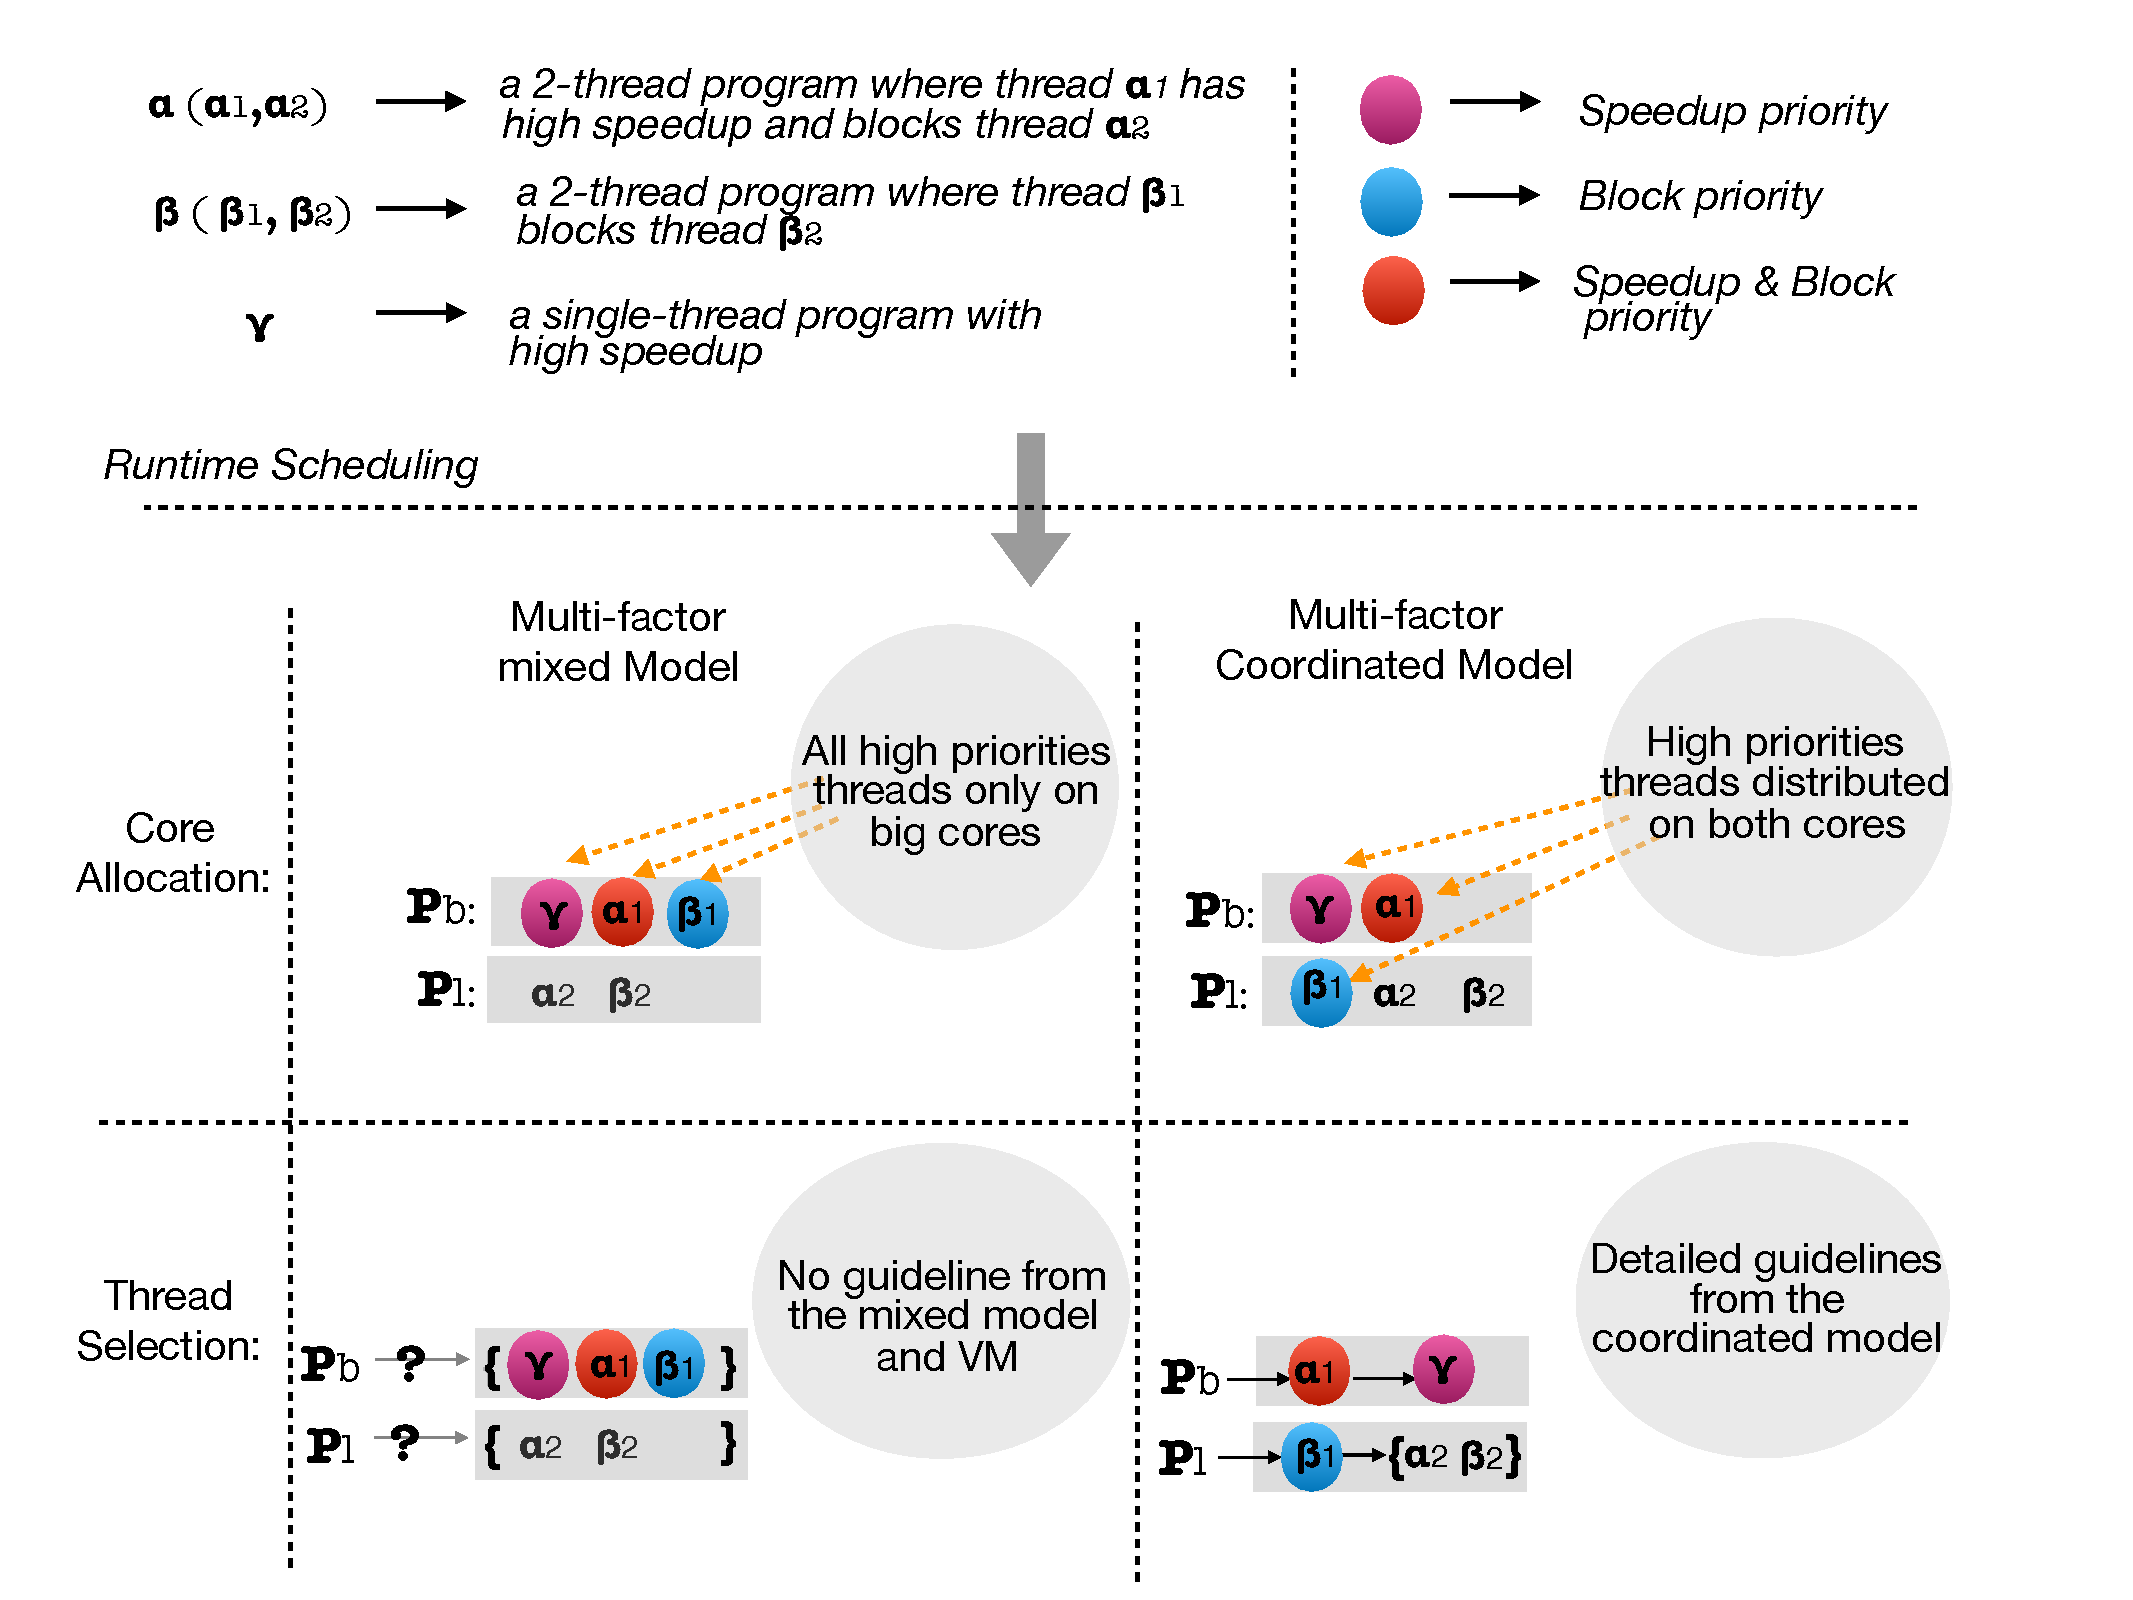
\includegraphics[scale = 0.26]{figures/me.pdf}
\caption{Motivating Example: Multi-threaded multiprogrammed workload on asymmetric multicore processors with one big core $P_b$ and one little core $P_l$. Controlling only core affinity results in suboptimal scheduling decisions.}
\label{me}
\end{figure} 

%In brief, fairness-oriented approaches have demonstrated their efficiency on multiprogram co-executed workloads with single-thread applications as precise mathematical analysis can be constructed \cite{kim2016fairness, kim2018exploring}. Bottleneck acceleration methods equipped with a runtime core sensitivity model have shown significant advantage on multi-thread applications in general single-program workloads \cite{joao2012bottleneck,joao2013utility}. In addition, with more emphasis posed on fairness with help of VM one can also obtain a powerful multi-factor mixed model applied by the state-of-the-art AMP-aware scheduler \cite{jibaja2016portable}. 

%To the best of knowledge, there are two problems remain in the VM-based multi-factor mixed model when it is targeting multi-thread multiprogram scheduling.   
%In brief, single-factor based approach can efficient deal with certain scenarios with limited workloads and runtime but losing generality. Multi-factor based approaches have been shown to be the trend to address general scheduling problem on AMPs with multi-thread workloads. 
%To the best of knowledge, there are two remain problems in the state-of-the-art multi-factor based approach:

\textbf{\textit{Motivating Example:}} To demonstrate the problem, consider the motivating example shown in Figure~\ref{me}. This AMP system has a high performance big core, $P_b$, and a low performance little core, $P_l$. Three applications, {$\alpha$, $\beta$, $\gamma$}, are being executed. $\alpha$ and $\beta$ have two threads.
The first thread of each application, $\alpha_1$ and $\beta_1$, blocks the second thread of their application, $\alpha_2$ and $\beta_2$ respectively. $\gamma$ is a single-threaded application. $\alpha_1$ and $\gamma$ enjoy a high speedup when executed on the big core, $P_b$. WASH~\cite{jibaja2016portable}, the existing state-of-the-art multi-factor heuristic, would likely assign the high speedup thread and the two blocking threads to the big core. The thread selector of $P_b$ has no information about the criticality of the threads assigned to it, so the order of execution depends on the underlying Linux scheduler.

A much better solution is possible if we control both core allocation and thread selection in a coordinated, AMP-aware way. In this case, we map the two threads that benefit the most from the big core, $\gamma$ and $\alpha_1$, to $P_b$, while we map the other bottleneck thread, $\beta_1$, to $P_l$. This will not impact the overall performance of $\beta$. The thread selector knows $\beta_1$ is a bottleneck thread and executes is immediately. So, what we lose in execution speed for $\beta_1$, we gain in not having to wait for CPU time. Similarly, this coordinated policy guarantees that $\alpha_1$ will be given priority over $\gamma$. 

%Based on the multi-factor mixed model \cite{jibaja2016portable}, either the high speedup thread ($\gamma$) or blocking threads ($\alpha_1,\beta_1$) will have affinity on $P_b$ -{\it local-optimal decision}. When the thread selector on $P_b$ is invoked, no more guideline can be obtained from the thread affinity provided by the mixed model - {\it loss of information with mixed priority}. Instead, a better solution can be provided in a multi-factor decentralized model by only mapping the two high speedup threads ($\gamma,\alpha_1$) to $P_b$ and keeping the other blocking thread $\beta_1$ in $P_l$ - {\it global-aware decision}. Then the thread selector invoked by both $P_b$ and $P_l$ guided through the blocking priority, will select and accelerate bottleneck threads $\alpha_1,\beta_1$ locally and simultaneously without waiting each other - {\it sufficient information with precise priority}.  

%both of them will get high priority and be affiliated on the big core. Thus, some of those high priority threads need to be waited in the runqueue of $p_b$. Further, when $p_b$ is ready to select the next task, it may select a $t_s$ first instead of a $t_b$ as the original bottleneck priority has lost after setup its affinity. In brief, the core allocator made the first {\it selfish} greedy decision to enqueue those high priority threads on big core without leaving a better solution space for thread selector. Second, the thread selector lose original information and cannot guarantee to make a good decision. With efficient preemption mechanism, $p_l$ can select a $t_b$ even from $p_b$'s runqueue, but this leads to additional overhead from migration. If the core allocator and thread selector can be collaborated, a trivial better solution in this example can be $p_b$ running \{$t_s \cap t_b$\} whilst $p_l$ running \{$t_b$\}. 

%The first problem is obvious as in runtime scheduling, every change in a current decision will influence the future solution space and there is no way to predict it especially for asymmetric multicore processors with multiple multi-thread workloads.  
%To demonstrate the second problem, scheduling a ready thread from a run-queue in big core to be executed in a ready little core can result in an optimal solution from a greedy point of view, or we say a {\it current} optimal solution. But if this thread will only run on the little core for a tidy bit of time and then move back to a big core by preemption when the big core is ready, the overall runtime overhead from additional migrations may totally defeat the benefit from the hard and useless work on the little core. A high level motivating example is shown in Fig \ref{mt}, where $\mathcal{T}$ is a high priority thread which just ranked in the second position under the current running thread on big core's run-queue. By global scheduling, a ready little core will decide to run this high priority thread $\mathcal{T}$ and migrate it from big core's run-queue. While the problem happens if the big core finish its current thread right after the migration issued by the little core, as the big core will decide to run $\mathcal{T}$ and move it back by preemption. Those frequent runtime selections and migrations do lower the performance in this case.

In this paper, we introduce COLAB, an OS scheduling policy for asymmetric multicore processors that can make such coordinated decisions. Our scheduler uses three collaborating heuristics to drive decisions about core allocation, thread selection, and thread preemption. Each heuristic optimizes primarily one of the factors affecting scheduling quality: core sensitivity, thread criticality, and fairness respectively. Working together, these multi-factor heuristics result in much better scheduling decisions.

We integrated COLAB inside the Linux scheduler module, replacing the default CFS policy for all application threads. We evaluated our policy on multiple big.LITTLE-like simulated systems running 36 distinct workloads, each workload being a random selection of PARSEC3.0, SPLASH2, and SPEC CPU2006 benchmarks. In almost all cases, COLAB was able to improve both turnaround time and throughput compared to the state-of-the-art and the Linux default. In the best case, turnaround time was 50\% less under our policy than under WASH and CFS.

%In brief, our proposed framework equipped with a multi-factor {\it decentralized} model - different runtime factors are distributed to be mainly addressed by different functional units of the scheduler, including core allocator, thread selector and preemption trigger. Decisions in each functional unit are directly guided by priorities from sufficient runtime without losing information through a mixed central model. Those decisions only aim to benefit each of their targeting factors and avoid making trouble for each other, so neither greedy nor local-optimal from a multi-factor point of view. Then all those sub-decisions from different functional units in scheduler dynamically collaborate together to result in overall smarter scheduling decisions during runtime. 

The main contributions of our work are:
\begin{itemize}
\item The first AMP-aware OS scheduler targeting general multi-threaded multiprogrammed workloads.
\item A set of collaborative heuristics for prioritizing thread based on core sensitivity, thread criticality, \emph{and} fairness.
\item Up to 50\% lower turnaround time, 5\% to 28\% on average, compared to the Linux CFS scheduler and WASH.
\end{itemize}

The remainder of this paper is presented as follows: Section 2 describes the background and related work. Section 3 presents our multi-factor collaborative model. We describe its implementation and analyze its operation in Section 4. We evaluate the scheduling police in Section 5, and we summarize and conclude the paper in Section 6.  

\section{Background and Related Work}
\label{rw}

\begin{table}
  \caption{Qualitative Analysis on Related Work}
  \center
  \label{rwt}
  \scalebox{0.8}{
   \begin{tabular}{p{3cm} p{1cm} p{1cm} p{1cm} p{2.2cm}c c c c c }
     \toprule[1pt]
     Approaches&Core Sens.&Fairness&Bottle- neck&Collaborative\\
     \toprule[1pt] 
    Kumar, et al \cite{kumar2004single} &$\checkmark$&&&\\
    Li, et al \cite{li2009efficient}&&$\checkmark$&&\\
    Suleman, et al. \cite{suleman2009accelerating}&&&$\checkmark$&\\
    Saez, et al. \cite{saez2012leveraging}&$\checkmark$&$\checkmark$&&\\
    Craeynest, et al. \cite{van2013fairness}&$\checkmark$&$\checkmark$&&\\
     Cao, et al. \cite{cao2012yin}&$\checkmark$&&&\\
     Joao, et al \cite{joao2013utility}&$\checkmark$&&$\checkmark$&\\
     Kim, et al \cite{kim2018exploring}&$\checkmark$&$\checkmark$&\\
     Jibaja, et al \cite{jibaja2016portable}&$\checkmark$&$\checkmark$&$\checkmark$\\
    \textbf{COLAB}&$\checkmark$&$\checkmark$&$\checkmark$&$\checkmark$\\
    \bottomrule
  \end{tabular}}
\end{table}

Initially described by Kumar et al.~\cite{kumar2004single,kumar2003single}, single-ISA heterogeneous multicore processors allow for more efficient processing, but to realize this we need the OS scheduler to match threads with cores more suited to their requirements. A straightforward way to determine good matches is based on the \emph{IPC} of the application on each kind of core. While easy to understand and perform, IPC is a reliable metric of performance only for single threaded applications, the search might be lengthy, and it will be affected by resource sharing and phase changes.

To work around some of these problems, other approaches have used performance models to predict the speedup due to executing a thread on another core type. Saez et al.~\cite{saez2012leveraging} build such a model based on \emph{ILP} and \emph{LLC miss rates}, Craeynest et al.~\cite{van2012scheduling} used \emph{CPI stack}, \emph{ILP}, and \emph{MLP}, while Jibaja et al~\cite{jibaja2016portable} applied Principal Component Analysis to select the performance counters most closely correlated with performance and built a linear model out of them. In all cases, the predicted speedup is used to decide \emph{Core Sensitivity}, how sensitive the thread's performance is on the type of core used. The more sensitive threads are assigned to high performance cores exclusively, the rest can be assigned to any type of core.

%\emph{Core sensitivity} has been a main concern since they come up with the AMPs - they executed threads on each type of cores and then used {\it IPC} to guide the selection. To build up a more precise model, more performance counters were considered to predict the relative speedup, such as $ILP$ and {\it LLC miss rates} applied by Saez, et al. \cite{saez2012leveraging} in their speedup factor estimation model and {\it CPI stack, ILP and MLP} by Craeynest, et al \cite{van2012scheduling} in their performance impact estimation (PIE). Addition helps from VM services have also been discussed and involved, as presented by Cao, et al. \cite{cao2012yin}. It provided a new opportunity of high-efficiency for AMPs scheduling by binding low priority tasks, such as VM helper threads, to the little cores. Furthermore, machine learning based approaches with the help of VM has been applied to further select performance counters and predict the speedup. As illustrated by Jibaja, et al. in \cite{jibaja2016portable}, principal component analysis is applied to select important performance counters from the initial comprehensive set and then regression is conducted to finalize the prediction model.

\emph{Acceleration of bottleneck and critical threads} is also necessary for high performance on AMPs. Kumar et al.~\cite{Kumar:2005:HCM:1100859.1100890} early on identified the benefit of executing Amdahl's serial bottlenecks on high performance cores, while executing parallel code in low performance, low power cores. Suleman et al.~\cite{suleman2009accelerating} proposed accelerating critical code sections too, in order to minimize the time a thread works on shared data and keep such data on the big core caches. Joao et al.~\cite{joao2012bottleneck,joao2013utility} generalized this idea by identifying and accelerating bottleneck functions dynamically. Using programmer hints and hardware support, they measure the number of cycles spent by each thread waiting on data from a (potentially) bottleneck function. If above a waiting cycle threshold, the function is accelerated. Jibaja et al.~\cite{jibaja2016portable} proposed finding bottleneck Java threads by measuring waiting time on contended locks.

Maintaining \emph{scheduling fairness} is an additional challenge introduced by AMPs. Fair schedulers try to balance the processing time given to each thread, process, or process group. Most implementations regard all sources of processing time as equivalent, which is not the case with AMPs. Li et al~\cite{li2007efficient} introduced asymmetry-aware load balancing where the load assigned to each core is proportional to its processing power. Craeynest et al.~\cite{van2013fairness} built an \emph{equal progress} scheduler. Using their performance model they were able to estimate the amount of small core processing time that each core should be given to progress as much as it has. The scheduler then prioritized threads so that the progress of all threads is the same. Multiple other scheduling heuristics have tried to maximize fairness on AMPs~\cite{zahedi2018amdahl,wang2016rebudget,kim2018exploring} but for restricted scheduling scenarios.

%In addition to the core sensitivity and speedup factor, AMPs also brought new challenges to keeping fairness during execution. The default Linux Completely Fair Scheduler (CFS) from kernel version v2.6.23 developed by Ingo Molnar \cite{molnar2007cfs} achieved complete fairness for multiprogrammed execution on a CPU. The underlining red-black tree structure and visual runtime {\it vruntime} based preemption mechanism kept multiprogrammed running in fairness progress without a timeslice setup or any heuristic needs. To deal with the challenge from AMPs, Li et al \cite{li2007efficient} designed framework to first schedule threads on high-performance cores and then keep  asymmetry-aware load balancing between AMPs. Followed by they involved distributed weight round-robin \cite{li2009efficient} to improve efficiency further and achieve high-scalable in addition of fairness on multicore processors. But the weight value in their approaches was only based on a default static priority of threads and no concern on the core sensitivity issue. Craeynest, et al. \cite{van2013fairness} proposed a AMP-oriented fairness model with a core sensitivity concern. Equipped with their previous PIE model to predict relative speedup as described above, they designed an $equal$-$progress$ fairness approach to keep multi-threaded programs running in relative equal progress on AMPs by updating their actual execution time based on predicted big-versus-small-core scaling factor from PIE. Jibaja, et al \cite{jibaja2016portable} achieved its equal progress by dynamic workload analysis and classification and then left the final scheduling decisions by CFS.
%More complex fairness metrics and model have been proposed recently, including the market-based models either by Zahedi, et al. \cite{zahedi2018amdahl} or Wang and Martinez \cite{wang2016rebudget} and the uniformity fairness scheduling by Kim and Huh \cite{kim2018exploring}. While those approaches were either only focusing on processor allocation instead of the runtime scheduling or targeting single-thread multiprogrammed  to build up their representation, for which the total amount of jobs for each thread is deterministic. So achieving a relatively equal progress is still the main concern for fairness on multi-threaded scheduling on AMPs. 

Among all previous work on AMP schedulers, only Kim and Huh~\cite{kim2018exploring} and Jibaja et al.~\cite{jibaja2016portable} targeted the general case of multi-threaded multi-programmed workloads. The uniformity fairness policy~\cite{kim2018exploring} focuses only on fairness and core sensitivity, without provision for bottleneck acceleration. WASH~\cite{jibaja2016portable} is the closest existing scheduler to ours. It handles core sensitivity, bottlenecks, and maintains fairness for the general scheduling case but controls only core affinity, leaving all other decisions to the baseline Linux scheduler. We use a WASH-like implementation for the Linux scheduler  as our state-of-the-art. A summary with qualitative comparison on the related work is shown in Table \ref{rwt}.

%The fact that Linux CFS results better than an AMP-aware scheduler like WASH in certain workloads is counter-intuitive. One reason is that some embarrassed parallel workloads do not need much synchronization/multi-threaded communication. So the blocking counter always output all-zero which is useless for decisions but increasing runtime overhead. Another reason is no much actual speedup for threads in some symmetric multi-threaded workloads when each thread are doing similar job with equally partitioned data. Speedup model is then inaccuracy and leads to bad heuristics with useless migrations

%Other recent AMP-aware schedulers either focusing on special targets, such as high-reliability by Naithani, et al. \cite{naithani2017reliability} and tail latency by Haque, et al. \cite{haque2017exploiting}, or on more complex AMPs with heterogeneous-ISA by Venkat, et al. \cite{venkat2014harnessing} which are beyond the scope of our general-propose work here. 


\section{Multi-factor Coordinated Scheduler}
We analyze the performance impact of multiple runtime performance factors and their relationships with different functional units in the scheduler. We build a scheduler which addresses these performance problems in a coordinated way.

\begin{figure}
\centering
\includegraphics[scale=0.45]{figures/mfa.pdf}
\caption{A diagram of Performance Factors and Relationships with Scheduling Functions}
\label{figure:f1}
\end{figure} 

\subsection{Runtime Factor Analysis}
The relationships between runtime performance factors and the functions which address them is shown in Figure~\ref{figure:f1}. In order to achieve runtime collaboration, both core allocator and thread selector share information and account for all measured performance factors, including core sensitivity, bottleneck acceleration and fairness carefully as illustrated below:
%We describe them below by discussing each element. 
%\begin{itemize}
\subsubsection{Core Allocator}
AMP-aware Core allocators are mainly directed by the core sensitivity factor -- migrating a high speedup thread (with a large differential between big and little core execution time) from  a little core to execute on a big core will generally provide more benefit than migrating a low speedup thread. 

However, this heuristic is overly simplistic. Issues are revealed when the bottleneck factor is considered simultaneously on multiprogrammed workloads. Previous approaches \cite{jibaja2016portable} simply combine the calculation from  bottleneck acceleration and predicted speedup together, but this can result in suboptimal scheduling decisions -- both locking threads and high speedup threads may be accumulating in the runqueues of big cores as is illustrated in the motivating example in the Introduction. More intelligent core allocation decisions can be made by avoiding a simple combination of bottleneck acceleration and speedup -- the overall schedule can benefit from a more collaborative execution environment where big cores focus on high speedup bottleneck threads, and little cores handle other low speedup bottlenecked threads without additional migration.

%migrating threads with a lower predicted speedup, but which are blocking other threads.  
Furthermore, core allocators are desired to achieving relative fairness on AMPs by efficiently sharing heterogeneous hardware and avoiding idle resource as much as possible. 
Simply mapping ready threads uniformly between different type of cores can not achieve true load-balancing -- the number of ready threads prioritized on different type of core is different and thus, a hierarchical allocation should be applied to guarantee the overall fairness, which avoids the need to frequently migrate threads to empty runqueues. 

\subsubsection{Thread Selector}
Thread selector makes the final decisions on which thread will be executed during runtime. It is usually the responsibility of thread selector to avoid bottlenecking by thread blocking. In a multi-thread multiprogrammed environment, multiple bottleneck threads from different programs may need to be accelerated simultaneously with constraint hardware resources. Instead of simply detecting the bottleneck threads and throwing all of them to big cores as previous bottleneck acceleration schedulers \cite{jibaja2016portable,joao2013utility,joao2012bottleneck}, the thread selector needs to make collaborative decisions -- ideally, both big cores and little cores select bottlenecks to run simultaneously.

Core sensitivity is usually unrelated to the thread selector -- whether a thread can enjoy a high speedup from a big core compared with a little core is unrelated to which runqueue it is on, or came from. Therefore the thread selector should separate thread priority caused by core sensitivity and solely base decisions on bottleneck acceleration. One exception is that when the runqueue of a big core is empty and the thread selector is invoked -- the speedup factors from core sensitivity of ready threads should be considered only in this case. Big cores may even preempt the execution of little cores when necessary.  

The final concern of thread selector is about fairness. Scaling time slice of threads by updating the time interval of thread selector has been shown to efficiently guarantee the equal progress \cite{van2013fairness} in multi-threaded single-program workloads and achieve fairness. 
%In single-threaded multiprogrammed scenarios, complicated fairness formulation \cite{kim2018exploring} has been proposed to guide the thread selector for more precise decisions. 
Problems occur when targeting multi-threaded multi-programmed workloads. Simply keeping a thread-level equal progress is not enough to guarantee the multi-application level fairness -- the thread selector should ensure the whole workload is in relative equal progress without penalizing any individual application. In fact,  multi-bottleneck acceleration by both big and little cores does provide an opportunity for this - the thread selector makes the best attempt to keep fairness on all applications by accelerating bottlenecks from all of them and as soon as possible.


%\textbf{\textit{Fairness:}} Fairness is critical for system performance. A good schedule achieving relative fairness on AMPs should efficiently share heterogeneous hardware and avoid idle resource as much as possible. To achieve the expected relative equal-progress between threads and load-balancing between cores, the core allocator should map ready threads relative uniformly,avoiding the need to frequently migrate threads to empty runqueues. The design of the preemption triggering mechanism  also affects fairness, as it determines the maximum length of a time slice.


%The preemption triggering mechanism of thread selector is also related with the fairness factor as it determines the slice of a task running each time - a thread currently running on big cores should have relatively shorter time slice against its running on little cores to result in similar progress.
%The preemption should be triggered and the thread selector should be invoked less frequent on little cores than on big cores     

%\textbf{\textit{Core Sensitivity:}} Previous approaches considered core sensitivity and predicated speedup of threads but can result in poor scheduling decisions on multi-threaded, multi-programmed co-execution workloads. Selecting threads simply by predicted speedup on asymmetric cores may not lead to a overall good solution --  for instance, a high speedup thread detected on a little core could benefit by migrating to a big core, but is not blocking a significant number of other threads. The overall schedule can benefit more by migrating threads with a lower predicted speedup, but which are blocking other threads. Thus, we find priority from core sensitivity should be mainly addressed by the core allocator and be independent from the thread selector. 
%For instance, a thread with high predicted speedup should have more opportunities to be allocated and executed on a high-performance big core compared to a low predicted speedup thread. Higher speedup and more sensitive on big core does not indicate any {\it emergency} to execute this threads amount all other ready threads during the runtime. 
%No priority should be given to high-speedup threads for a thread selector, only if in a special case when a big core finishes its current task with an empty runqueue and all other big cores hold empty runqueue as well - so it needs to globally select a ready thread from a runqueue of little core and then relative higher speedup threads are better candidates. This special case won't even appear in large-scale parallel workloads scenarios where the number of co-executing programs is at least greater than the number of cores - there will always be waiting threads in a big core's runqueue based on fairness core allocation as no data-dependence between threads from different programs. 

%\textbf{\textit{Bottleneck Acceleration:}} Threads from multi-threaded programs holding contended locks and blocking other parallel threads should be identified as bottleneck and be executed as soon as possible. In large-scale workloads scenarios where multi-threaded multi-program are co-executing on limited AMPs resources and multiple blocking threads waiting to be executed simultaneously, the thread selector should take the main duty to select those bottlenecks and run the corresponding critical code segments in an efficient way without confused by the priority from core sensitivity. In detail, the thread selector triggered by big cores should always give higher priorities for a thread with higher blocking level against another thread with higher speedup level and lower bottleneck. It may preempt the running threads on little cores to accelerate them when suited. The thread selector triggered by little cores should also intend to select relative high blocking threads and accelerate them locally first, instead of trivially migrating it to big cores and waiting to be actual accelerated there.  

\begin{figure}
\centering
\includegraphics[scale=0.57]{figures/COLAB_M.pdf}
\caption{Coordinated Model by Multi-factor Collaboration}
\label{figure:f2}
\end{figure} 

\subsection{Collaboration}
To address the problems detailed above, we designed a coordinated multi-factor scheduler in which the core allocator and the thread selector collaborate to achieve high performance and high fairness, when compared to the state-of-the-art mixed multi-factor evaluator in WASH \cite{jibaja2016portable}.
%While the way we define whether a thread's relative speedup value is high or low is similar as in WASH based on hardware configuration - if we have same number of big and little cores, then we rank all ready threads based on its relative speedup and view the first half as high speedup value. 
The flowchart of our model is shown in Figure~\ref{figure:f2}. 
Collaboration is facilitated by periodically labeling ready threads in two different categories, based on runtime models of speedup prediction and bottleneck identification: 
%\begin{itemize}
\subsubsection{Labels for Core Allocation}
Threads with high predicted speedup between big and little cores will be labeled as high priority on big cores. Threads with both low predicted speedup and blocking levels -- non-critical threads -- will obtain high priority on little cores (and low priority on big cores). Remaining threads obtain equal priority on either big or little cores -- these threads can then be allocated freely to balance the load of cores.
\subsubsection{Labels for Thread Selection}
Threads with high blocking level will be labeled as high priority on local thread selection. The same priority will be given on these blocking threads whether the issuing cores are big or little, so the labels of thread selection do not distinguish the type of cores.The label nevertheless records the type of the current core -- threads always have priority to be selected by the same type of cores if there exists a core of the same type with an empty runqueue. Running threads on little cores are also labeled as they may be preempted to migrate and execute on big cores when suited, but running threads will never have priority over waiting ready threads. 


%The thread labels should be not only be based on the relative ranking between threads, but also on boundary conditions targeting different hardware resource and experimental environments. 
%We setup empirical boundaries for speedup and blocking: (1) No thread is ranked as high-speedup if its predicted speedup value is less than an empirical architecture-specific boundary, calculated using relative frequency between big and little cores. 

%For instance, if the big cores' frequency is 2x faster than the little cores and ready threads get around 1.5x predicted speedup, this likely means threads haven't be executed long enough to get a more precise speedup value and we should not bind or migrate any thread at this step. 
%(2) Threads will not be ranked as high-blocking if the rate of their blocking time and life time are less than a relative boundary or the life time of them are less than a starting point - For instance, no thread should be ranked as relative high-blocking during the initial time periods of experiments.   
%It is mainly benefit in a mixed workloads scenario where we co-execute single and multi-threaded multiprogrammed - a non-computing-intensive code segment from a single thread program can neither enjoy good performance gain on big cores nor block others. So we should better keep it in a little core and let other blocking threads to be executed before it. 

After the labeling process, fairness, core sensitivity and bottleneck acceleration are represented by labels on threads can be handled by either the core allocator or the thread selector or both together. Based on this coordinated model, the core allocator and thread selector handle different priorities queues from the set of ready threads -- their decisions are not greedy on a mixed multi-factor ranking like WASH, rather provide a collaborative schedule.

Another important issue handled by the collaborative multi-factor model is to ensure relative equal-progress of threads as shown in the upper-right corner of Figure~\ref{figure:f2}. Instead of interfering with the priority and decisions of thread selection, we achieve equal progress in threads by our scaled time slice approach, based on the predicted speedup value of threads running on big cores. The slices of threads on big cores are relative shorter than on little cores. The thread selection function is triggered more often to swap executing threads on big cores, which guarantees the relative equal-progress of threads executed on all cores.

The runtime model periodically extracts the performance counters, which represents the current execution environment of multi-threaded multi-programmed workloads on the AMPs. The model then computes the updated runtime factors, including the predicated speedup value and blocking counts. This information is attached to the threads and reported back to the multi-factor labeler for next round. We present our runtime model implementations in the section below. 

\section{Runtime Design and Implementation}
We implement our approach on the GEM5 simulator \cite{binkert2011gem5}, modifying the simulator and constructing interfaces between the Linux kernel v3.16 with the CFS scheduler.

\subsection{Runtime Factors Implementations}
To implement the runtime multi-factor model, we update the main scheduler function \texttt{\_\_sched\_\_schedule()} of the Linux kernel by adding a thread labeling process as described in section 3.2 above. The similar method is applied when we re-implement the WASH scheduler by updating thread affinities without the help of VM. 

We present our implementation of the performance analyses we use to achieve optimization:

\textbf{\textit{Machine Learning based Speedup Prediction:}} Predicting relative speedup of each thread on heterogeneous cores is a core functionality of any core sensitivity aware scheduler targeting AMPs. Our implementation of the speedup model follows the common approach in the literature \cite{van2013fairness,jibaja2016portable,saez2012leveraging}- an off-line trained predictive model applying on on-line. 

To construct the training set, we run all applications in single-program mode with two basic SMP configurations - full little cores and full big cores. We compute the speedup of each application between the heterogeneous cores and record all 225 performance counters from the simulated ARM cores in detailed CPU model from GEM5 \cite{binkert2011gem5} in full big core execution. The Principal Component Attribute Transformer (PCAT) technique \cite{witten2016data} is applied to select six performance counters for use as features from the initial larger set. We choose six performance counters, plus a counter of committed instructions (used for normalization) as this is a typical number implemented in real hardware, such as Intel Sandy Bridge \cite{jibaja2016portable}. Finally, linear regression is applied on the applications set with selected counters and actual speedup to train the weight value of each counter. The selected counters and predictive linear speedup model targeting ARM big.LITTLE processors running on GEM5 are shown in table \ref{pca_sp}.  

\begin{table*}
  \caption{Selected performance counters and Speedup Model}
  \center
  \label{pca_sp}
   \scalebox{1}{
   \begin{tabular}{p{2cm} | p{6cm} | p {9cm} c c c}
 % \begin{tabular}{l c c c c}
  \hline
    \multicolumn{3}{c}{Selected GEM5 performance counters by PCAT}\\
  \hline
     Index&  Name& Description \cite{binkert2011gem5} \\
    \hline
     A: & fp\_regfile\_writes & number of integer regfile writes\\
     B: & fetch.Branches & number of branches that fetch encountered\\
     C: & rename.SQFullEvents & number of times rename has blocked due to SQ full\\
     D: & quiesceCycles & number of cycles  quiesced or waiting for an interrupt\\
     E: & dcache.tags.tagsinuse & cycle average of tags of dcache in use\\
     F: & fetch.IcacheWaitRetryStallCycles & number of stall cycles due to full MSHR\\
     \hline
     G: & commit.committedInsts & number of instructions committed\\
     \hline
    % \toprule[1pt]
     \multicolumn{3}{c}{Linear predictive speedup model}\\
     \hline
     \multicolumn{3}{c}{2.6109+((0.0018*-0.185A)+(0.0259*0.187B)+(0.1047*0.194C)+(-0.023*0.238D)+(0.0492*-0.299E)+(-0.1388*-0.227F))/G}\\
  %  \bottomrule
  \hline
  \end{tabular}}
\end{table*}



\textbf{\textit{Bottleneck Identification:}}
On modern Linux systems synchronization primitives are almost always implemented using kernel futexes, regardless of the threading library used. Futex-based mechanisms use a single atomic instruction in user space to acquire or release the futex, if it is uncontested. Otherwise, it triggers a system call which forces the thread to sleep or wakes up sleeping threads, respectively.

This gives us a convenient single point where we can monitor blocking patterns between threads. We first add code in \texttt{futex\_wait\_queue\_me()} and \texttt{futex\_lock\_pi()}, right before the active thread starts waiting on a futex. We record the current time and store it in the \texttt{task\_struct} of the thread. We then insert code in \texttt{wake\_futex()} and \texttt{wake\_futex\_pi()}, right before the waiting task is woken up by the thread releasing the futex. There we calculate the length of the waiting period and we accumulate it in the \texttt{task\_struct} of the thread releasing the futex. This way we are able to measure the cumulative time each thread has caused other threads to wait. We use this as our metric of thread criticality for the rest of the paper.

\textbf{\textit {Speedup based Scale-slice Preemption:}} Although we implement our scheduler on Linux kernel by fully re-writing both the core allocator and thread selector, the underlining preemption mechanism of Linux is applying the virtual runtime {\it vruntime} in CFS with red-black tree data structure - whenever a new task is enqueued, a preemption wake-up function is invoked to check whether the new coming task should preempt the current task by computing the difference in vruntime and comparing with a boundary. 

To achieve relative equal-progress on AMPs, threads running on different types of cores should have different time slices instead of trying to achieve complete fairness on time. We update the default preemption wake-up function \texttt{wakeup\_ preempt \_entity()} in Linux by constructing an interface to the GEM5 simulator. We apply our runtime speedup model to update the vruntime of the current task by dividing it by the thread's speedup value if the triggering core is a big core. The ensures relative equal progress.




\subsection{Scheduling Algorithm Design and Implementation}
\begin{algorithm}
\caption{Collaborative Multi-factor Scheduler targeting Asymmetric Multicore Processors}
\label{alg:1}
\begin{algorithmic}[1]
\STATE core\_alloctor\_(thread\_struct\ $t$)\{
%\FOR {$t : ready\_threads$}
%\IF {t->high\_speedup() \& t->high\_block()}
\IF {t.high\_speedup}
\RETURN rr\_allocator\_(big\_cores)
\ENDIF
\IF {t.low\_speedup \& t.low\_block}
%\& !unique(t->tgid)}
\RETURN rr\_allocator\_(little\_cores)
\ENDIF
\RETURN rr\_allocator\_(cores)
\STATE \}
\STATE thread\_selector\_(core\_struct\ $c$)\{
%\IF {c->cur \& !(preempt_wakeup)}
\IF {!empty(c.rq)}
\RETURN max\_block\_(c.rq)
\ENDIF
%\IF {c->type == big}
\IF {!empty(c.sched\_domain.rq)}
\RETURN max\_block\_(c.sched\_domain.rq)
\ENDIF
\IF {c.cpu\_mask == big}
%\FOR {t : little\_core->cur}
%\STATE candidates.enqueue(t)
%\IF {!empty(candidates)}
\RETURN  max\_block\_(c.sched\_domain\_little.cur)
\ENDIF
%\ENDFOR
%\ENDIF
%\FOR {t : other\_little\_core->rq}
%\STATE candidates.enqueue(sorted\_speedup(t))
%\ENDFOR
%\IF {!empty(candidates)}
%\RETURN  max\_block\_(candidates)
%\ENDIF
%\ENDIF
%\FOR {t : other\_core->rq}
%\STATE candidates.enqueue(reversed\_speedup(t))
%\ENDFOR
\RETURN idle
\STATE \}
\end{algorithmic}
\end{algorithm}

Our scheduling algorithm is implemented by fully overriding the default task selector \texttt{pick\_next\_task\_fair()} and core allocator \texttt{select\_task\_rq\_fair()} in Linux kernel supported by the runtime factors. The pseudo-code of our scheduling algorithm is shown in Alg. \ref{alg:1}. 
Similarly to commonly used Linux notations, we use $rq$ to represent runqueue and $cur$ to represent the current task of a core in our code. We describe the two main functions below:

\textbf{\textit{Hierarchical Core Allocator:}}
When a thread is ready to be executed, whether it was just spawned for woken, the core allocator will be invoked to allocate this thread to a possible core's runqueue. To achieve relative load balancing and consider the influence from core sensitivity factor, we involve a hierarchical round-robin mechanism \texttt{rr\_allocator\_()}. Indicated by the speedup and blocking labels, threads are allocated to different core groups. Threads with high speedup level will be round-robin allocated in big core clusters (line 3). Low speedup and low blocking thread will only be allocated in round-robin over the little core clusters (line 5). 
%A technical issue here is we need to distinguish threads which are part of a multi-thread program from from single-thread programs - these single-thread program threads will definitely not block others and may not have a high speedup but we should nevertheless not bind them to little cores. They can be easily detected by the allocator by checking whether there are ready threads whose group pid (t->tgid) equals to any others (line 5). 
To fill the gap of different core clusters, remain ready threads (usually with normal speedup level and tiny block) will be relatively equally allocated to both core types by \texttt{rr\_allocator\_(core)} - this final round-robin shares counters with the first two big/little core specific round-robin to achieve overall load balancing (line 6).  

\textbf{\textit{Biased-global Thread Selector:}}
The thread selector is based on the principle of accelerating the most critical/blocking thread as soon as possible, shown in line 10, 12, 14. Triggered by different cores, the selector always try to return  a local candidate first instead of invoking additional migrations (line 10). When there are no local waiting threads and migration is beneficial, cores give priority for candidate threads waiting on other's runqueue and from there the most blocking thread will be selected.
To reduce the overhead of accessing global CPUs states, we follow the same principle of the default Linux CFS scheduling domain (\texttt{struct sched\_domain}) - returning the best candidate thread from the local core group first (line 12).
Further, we allow a big core to select and preempt a running thread on little core to accelerate it (line 13,14). Idle resources will only occur when there is not any possible useful work to be done (line 15) - for instance, we do not allow a little core to preempt a big core's execution. 
In summary, the thread selector can still access all other global runqueues when necessary, but it is biased to access nearly runqueues first, due to bottleneck and core sensitivity concerns. 
Note that the relative equal-progress for achieving fairness is addressed by the scale-slice preemption checker instead of the thread selector -- we give each thread a maximum time slice relative to its expected performance on the asymmetric core.

\textbf{\textit{Discussion:}}
This section provides a case study, implementing our scheduling framework targeting simulated ARM architectures and processors on GEM5.  However, the underlining general procedure and model can be implemented on real processors by using their hardware performance monitor events (PMU). All hardware counters used by our model are supported by the ARM Cortex-A57/A53 \cite{ARMA57} PMU.
%For instance, we input 150 PMU events \cite{ARMA57} of ARM Cortex-A57/A53 to the PCA process to build up corresponding speedup model when implement on real ARM cores.
%To further minimize the overhead of accessing global CPUs states to implement our approach on real systems, the thread selector can be configured to check other cpus one by one instead of 


\section{Experimental Evaluation}

\subsection{Experimental Setup}

 \begin{table*}
  \caption{Benchmarks Characteristics \cite{bienia08characterizationreport}\cite{woo1995splash}\cite{southern2016analysis}}
  \center
  \label{BC}
   \scalebox{1}{
   \begin{tabular}{ p{3cm} | p{3cm} | p{3cm} | p{3cm} | p{3cm} }
     \toprule[1pt]
     Name & Type of Parallelism & Synchronization Rate & Comm/Comp Ratio & Number Threads \footnote{$n$ is the input parameter.} \\
     \toprule[1pt]
    blackscholes & data-parallel & low & high & 1 + n \\
    bodytrack & data-parallel & medium & high & 2 + n\\
    dedup & pipline & medium & high & 3 + 3n\\
    ferret & pipline & high & medium & 3 + 4n\\
    fluidanimate & data-parallel & very high & low & 1 + n\\
   % freqmine & data-parallel & high & high &4\\
    swaptions & data-parallel & low & low & 1 + n\\
    radix & data-parallel & low & high & n\\
    lu\_ncb & data-parallel& low & low & n \\
    lu\_cb & data-parallel& low & low & n\\
    ocean\_cp & data-parallel & low & low & n\\
    water\_nsquared & data-parallel& medium & medium & n\\
    water\_spatial & data-parallel& low & low & n\\
    fmm & data-parallel& medium & low & n\\
    fft & data-parallel& low & high & n\\
      \midrule
     \bottomrule
  \end{tabular}}
\end{table*}

 \begin{table*}
  \caption{Benchmarks Compositions New}
  \center
  \label{BCN}
   \scalebox{1}{
   \begin{tabular}{ p{2cm} | p{7cm} | p{4cm} | p{2cm} }
     \toprule[1pt]
     \multicolumn{4}{c}{Synchronization-intensive VS Non-synchronization-intensive Workloads}\\
     \midrule
     Index & Workload Composition & Synchronizations & Threads \\
     \toprule[1pt]
    Sync - 1 & water\_nsquared - fmm & intensive & 4 \\
    Sync - 2 & dedup - fluidanimate & intensive & 18 \\
    Sync - 3 & water\_nsquared - fmm - fluidanimate - bodytrack & intensive & 9 \\
    Sync - 4 & dedup - ferret - fmm - water\_nsquared & intensive & 20\\
      \midrule
    NSync - 1 & radix - fft & non-intensive & 4 \\
    NSync - 2 & blackscholes - swaptions & non-intensive & 16 \\
    NSync - 3 & radix - fft - water\_spatial - lu\_cb & non-intensive & 8\\
    NSync - 4 & blackscholes - ocean\_cp - lu\_ncb - swaptions & non-intensive & 20\\
   %  \bottomrule
      \toprule[1pt]
     \multicolumn{4}{c}{Communication-intensive VS Computation-intensive Workloads}\\
     \midrule
     Index & Workload Composition & Comm/Comp & Threads \\
     \toprule[1pt]
    Comm - 1 & water\_nsquared - fft & Communication-intensive & 4 \\
    Comm - 2 & radix - blackscholes &  Communication-intensive & 16 \\
    Comm - 3 & water\_nsquared - fft - radix - blackscholes &  Communication-intensive & 8 \\
    Comm - 4 & bodytrack - dedup - ferret - fft &  Communication-intensive & 20\\
      \midrule
    Comp - 1 & water\_spatial - fmm & Computation-intensive & 4 \\
    Comp - 2 & fluidanimate - swaptions & Computation-intensive & 16 \\
    Comp - 3 & lu\_ncb - fmm - water\_spatial - lu\_cb & Computation-intensive & 8\\
    Comp - 4 & fluidanimate - ocean\_cp - lu\_ncb - swaptions & Computation-intensive & 20\\
     \bottomrule
     
  \end{tabular}}
\end{table*}

 \begin{table*}
  \caption{Workloads Compositions}
  \center
  \label{WC}
   \scalebox{0.9}{
   \begin{tabular}{p{1.5cm} |p{5.5cm} || p{1.5cm} |p{9cm} }
     \toprule[1pt]
     \multicolumn{4}{c}{Random-mixed Workloads from PARSEC3.0 and SPLASH-2}\\
     \toprule[1pt] 
    2B-1 &blackshcoles - radix &4B-1 &blackshcoles - bodytrack - radix - lu\_ncb\\
    2B-2 &fft - swaptions &4B-2 &water\_spatial - fmm - fft - fluidanimate\\
    2B-3 &lu\_cb - dedup  &4B-3 &lu\_cb - water\_nsquared - fmm - freqmine\\
    2B-4 &lu\_ncb - bodytrack &4B-4 &lu\_cb - lu\_ncb - bodytrack - dedup\\
    2B-5 &ferret - fluidanimate &4B-5 &radix - lu\_ncb - lu\_cb - fft\\
    2B-6 &freqmine - water\_nsquared &4B-6 &blackscholes - bodytrack - dedup - fluidanimate\\
    2B-7 &ocean\_cp - fft &4B-7 &radix - ocean\_cp - blackscholes - swaptions\\
    2B-8 &ferret - water\_spatial &4B-8 &water\_spatial - water\_nsquared - ferret - freqmine\\
    2B-9 &fluidanmiate - fmm &4B-9 &fmm - water\_spatial - ferret - swaptions\\
    2B-10 &fmm - water\_spatial &4B-10 &ocean\_cp - fft - fluidanimate - swaptions\\
  %  6B-M &blackshcoles,bodytrack,dedup,radix,lu\_ncb,lu\_cb\\
  %  8B-M &blackshcoles,bodytrack,dedup,fluidanmiate,radix,lu\_ncb,lu\_cb,radiosity\\
  %  12B-M &blackshcoles,bodytrack,dedup,fluidanmiate,streamcluster,swaptions,radix,lu\_ncb,lu\_cb,radiosity,ocean\_cp,fft\\    
     \midrule
 %    \toprule[1pt]
 %    \multicolumn{4}{c}{Multi/Single-thread multiprogrammed Workloads from PARSEC3.0, SPLASH-2 and SPEC2006}\\
 %    \toprule[1pt]  
 %   3B-1 &blackshcoles - radix - mcf &6B-1 &blackshcoles - bodytrack - radix - lu\_ncb - mcf - bzip2\\
  %  3B-2 &fft - swaptions - mcf &6B-2 &fft - radix - blackscholes - fluidanimate - mcf - bzip2\\
   % 3B-3 &freqmine - swaptions - mcf &6B-3 &blackscholes - dedup - freqmine - swaptions - mcf - bzip2\\
%    3B-4 &blackscholes - freqmine - bzip2 &6B-4 &lu\_cb - lu\_ncb - bodytrack - dedup - mcf - bzip2\\
    %3B-5 &ocean\_cp - fluidanimate - mcf &6B-5 &radix - lu\_ncb - lu\_cb - fft - mcf - bzip2\\
 %   3B-5 &radix - lu\_ncb - bzip2 &6B-5 &radix - lu\_ncb - lu\_cb - fft - mcf - bzip2\\
  %  3B-6 &fluidanimate - freqmine - bzip2 &6B-6 &blackscholes - freqmine - swaptions - fluidanimate - mcf - bzip2\\
   % 3B-7 &blackscholes - fluidanimate - bzip2 &6B-7 &lu\_ncb - ocean\_cp - bodytrack - swaptions - mcf - bzip2\\
%    3B-8 &dedup - fluidanimate - bzip2 &6B-8 &lu\_cb - ocean\_cp - dedup - swaptions - mcf - bzip2\\
 %   3B-9 &lu\_cb - swaptions - bzip2 &6B-9 &ocean\_cp - fft - fluidanimate - swaptions - mcf - bzip2\\
 %   7B-MS   &blackshcoles,bodytrack,dedup,radix,lu\_ncb,lu\_cb,mcf\\
 %   11B-MS &blackshcoles,bodytrack,dedup,canneal,swaptions,radix,lu\_ncb,lu\_cb,radiosity, bzip2,mcf\\ 
  %  15B-MS &blackshcoles,bodytrack,dedup,fluidanmiate,streamcluster,canneal,swaptions,radix,lu\_ncb,lu\_cb,radiosity, ocean\_cp,fft,bzip2,mcf\\   
  % &6B-7 &radix - ocean\_cp - blackscholes - swaptions - mcf - bzip2\\
    \bottomrule
  \end{tabular}}
\end{table*}

\textbf{\textit{Experimental Environment:}} We ran our experiments on GEM5, simulating an ARM big.LITTLE-like architecture. The big cores are similar to out-of-order 2 GHz CortexA57 cores, with a 49 KB L1 instruction cache, a 32 KB L1 data cache, and a 2 MB L2 cache. The little cores are similar to in-order 1.2 GHz CortexA53 ones, with a 32 KB L1 instruction cache, a 32 KB L1 data cache, and a 0.5 MB L2 cache. We evaluated two distinct hardware configurations, one with two big and two little cores and one with four big and four little ones. The OS is Linux v3.16. We cross-compiled the kernel with gcc v5.4.0, while we compiled the benchmarks inside the emulated environment with gcc v4.8.2.

\textbf{\textit{Workloads:}} For our workloads we used 17 different benchmarks. Fifteen are multi-threaded pulled either from PARSEC3.0~\cite{bienia11benchmarking} ({\it blackscholes, bodytrack, dedup, swaptions, freqmine, ferret and fluidanmiate}) or from SPLASH2~\cite{woo1995splash} ({\it radix, lu\_ncb, lu\_cb, ocean\_cp, water\_nsquared, water\_spatial, fmm and fft}). We added another two single-threaded benchmarks ({\it mcf, bzip2}) from SPEC CPU2006~\cite{henning2006spec} to complicate scheduling decisions. All benchmarks use pthread-based parallelism apart from \emph{freqmine} which does not support pthreads, only OpenMP. To keep the simulation time reasonably short, we use the \emph{simsmall} inputs for the multi-threaded benchmarks.

For \emph{mcf} we use the reference input, while for \textit{bzip2} we used the source reference input. We edited the source files of \textit{mcf} and \textit{bzip2} to limit the number of iterations of their outermost loops to 3000 for the former and 250 for the latter, to keep their runtimes in the same order of magnitude as the multi-threaded benchmarks.

%It is a common issue that GEM5 simulator does not support all PARSEC3.0 benchmarks well \cite{endo2014micro}, so we also applied several more SPLASH2 benchmarks \cite{woo1995splash}: {\it radix, lu\_ncb, lu\_cb, ocean\_cp and fft}. We also considered two more single-thread benchmarks ({\it mcf, bzip2}) from SPEC2006 \cite{henning2006spec} to make the tested multiprogrammed workloads further complicated. 
We randomly mix our selected benchmarks to build workloads with either multiple multi-threaded applications or mixed multiple multi-threaded and single-thread applications. Table~\ref{WC} shows the workloads we used. For all workloads, we boot the simulated system, start the benchmarks, and wait until they reach the end of their initialization. This is done with fast simulation. When all benchmarks are initialized, we switch to cycle accurate simulation and resume the execution of the benchmarks. We only collect statistics for the cycle accurate part of the simulation.

Each one of our results represents the average over two simulations with different core orders - either big cores first or little cores first. The initial state of the system can have a significant impact on performance. For the Linux scheduler in particular, the order of starting benchmarks will decide which benchmarks will be initially assigned to big and little cores. By randomizing the initial state and especially the execution order of the workload benchmarks for each simulation, we minimize the effect of randomness on our evaluation.

%The number of parallel threads for benchmarks from SPLASH2 can be setup easily as in input arguments, while for PARSEC benchmarks, we only setup the lower bound of threads and the program will then determines the actual number of threads based on the relationships described in \cite{southern2016analysis}. To avoid dominating system performance by a single benchmark in each workload, we normalized the number of threads from different benchmarks to be similar and keep the input sizes of all applications to be {\it simsmall}. 
%The only exception is on benchmark {\it streamcluster} from PARSEC3.0 - it is a known issue \cite{southern2016analysis,roth2012deconstructing} that increasing the number of threads to be greater than 4 will significantly decrease the performance of this benchmark because of its barrier based synchronization.

\textbf{\textit{Metrics:}} Our evaluation uses two metrics to quantify scheduling efficiency: {\it Heterogeneous Average Normalized Turnaround Time} (H\_ANTT) and {\it Heterogeneous System Throughput} (H\_STP). They are based on ANTT and STP, as introduced in~\cite{eyerman2008system}. For an application mix, both ANTT and STP use the runtime of each application when executed on its own, i.e. when there is no resource sharing and scheduling decisions have little effect. ANTT expresses the average slowdown of all applications in the mix, with the slowdown for each application being relative to its isolated runtime. STP expresses the sum of the relative throughputs for all applications, again relative to the isolated throughput.

For AMPs, these two metrics fail to work as intended. The runtime when executed alone is still affected by scheduling decisions, e.g. which threads to run on big cores. To overcome the problem, our modified metrics H\_ANTT and H\_STP use the runtime of each application in the mix when executed alone \emph{on a system where there are only big cores}. If the turnaround time of each application $i$ while being co-scheduled is $T^{M}_i$ and the turnaround time for the same application when running alone on a big-only system is $T^{SB}_i$, then:

$$ H\_ANTT = \frac{1}{n}\sum^{n}_{i=1}\frac{T^{M}_i}{T^{SB}_i}$$
$$ H\_STP = \sum^{n}_{i=1}\frac{T^{SB}_i}{T^{M}_i}$$

When we evaluate a single benchmark on its own, we use the {\it Heterogeneous Normalized Turnaround Time} (H\_NTT):

$$ H\_NTT = \frac{T^{M}}{T^{SB}}$$

H\_ANTT and H\_NTT are better when lower, H\_STP is better when higher. For most figures, we further normalize our results relative to the Linux CFS results for the same configuration and workload.

\textbf{\textit{Schedulers:}}
We compare COLAB against the Linux CFS scheduler~\cite{molnar2007cfs} and a scheduler based on WASH~\cite{jibaja2016portable}. WASH is implemented inside a Java VM and is meant to control the affinities of Java threads only. Our implementation uses the same heuristic as the original WASH but is part of the Linux scheduler and controls all application threads. Additionally, we replaced the WASH core sensitivity model with one built from scratch for our hardware configuration and our set of performance counters, using the same process as described in the WASH paper.

\begin{figure}
\centering
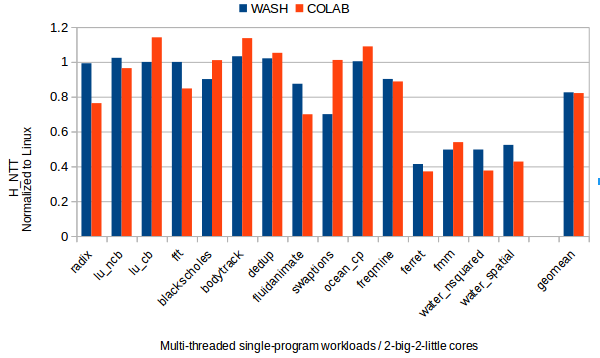
\includegraphics[scale=0.42]{figures/MSW4.png}
\caption{Heterogeneous Normalized Turnaround Time (H\_NTT) of single program workloads.  All results are normalized to the Linux CFS ones. Lower is better}
\label{MSW}
\end{figure}  
\begin{figure*}
\centering
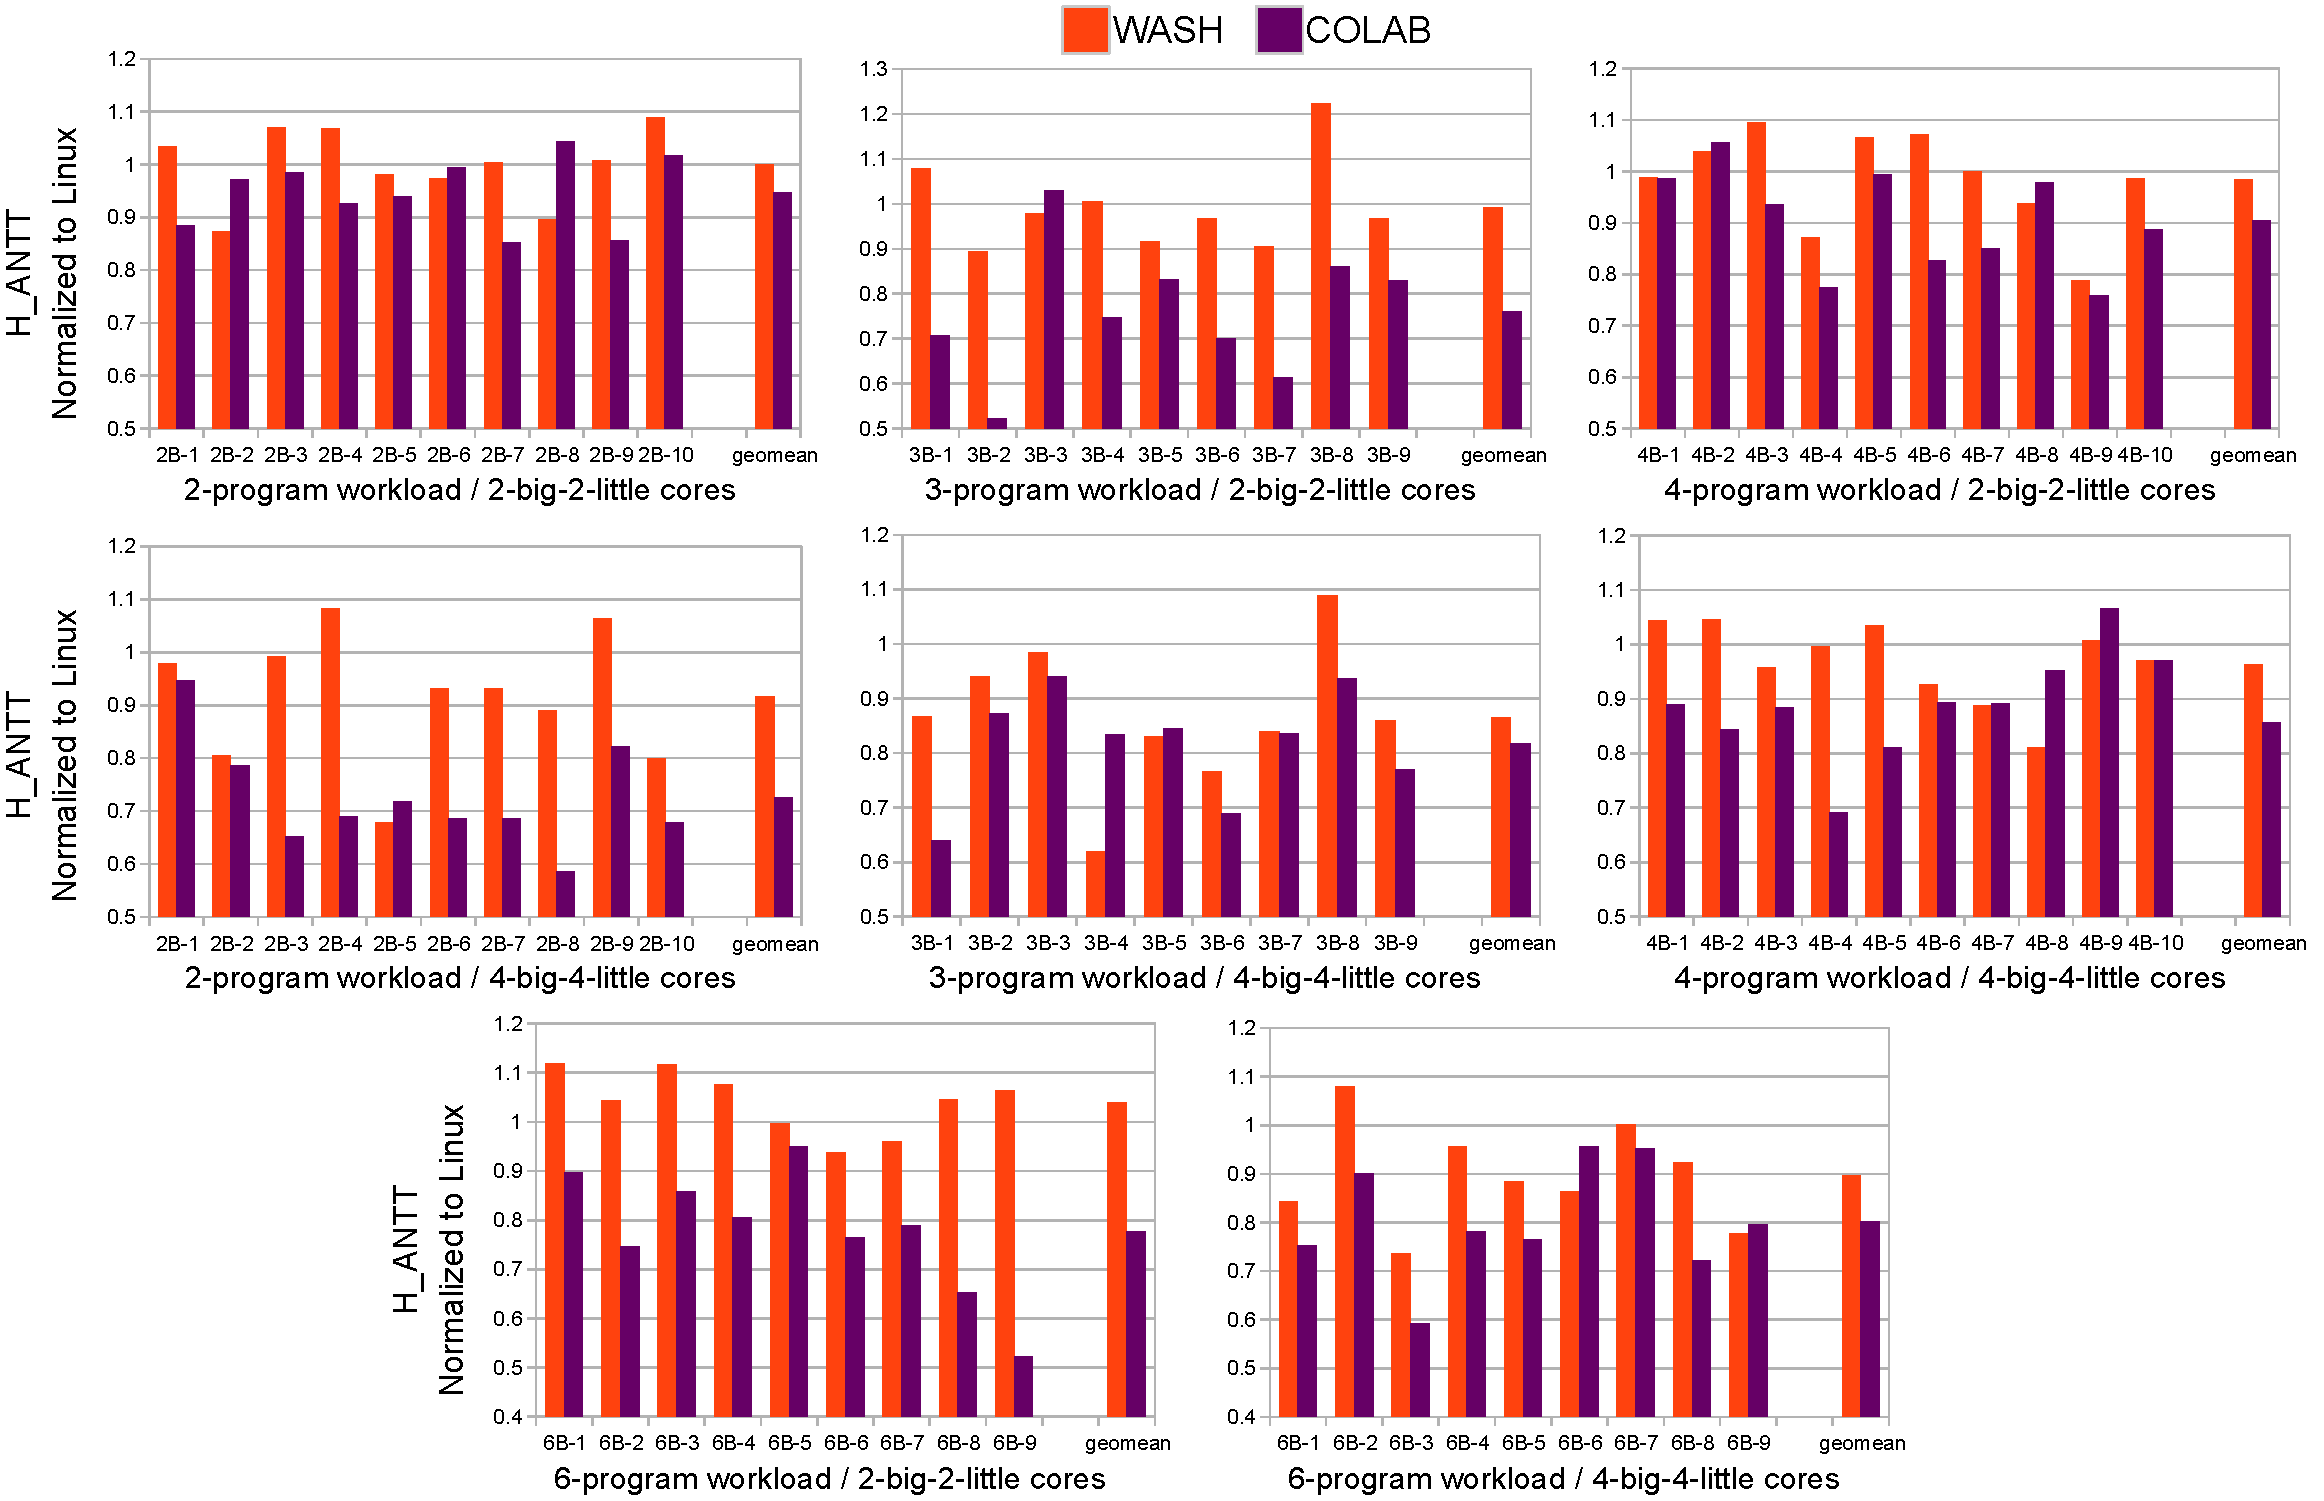
\includegraphics[scale=0.4]{figures/HANTT_NEW.pdf}
\caption{Heterogeneous Average Normalized Turnaround Time (H\_ANTT) of multiprogrammed workloads on 2-big-2-little and 4-big-4-little configurations. All results are normalized to the Linux CFS ones. Lower is better.}
\label{M24W}
\end{figure*}


\subsection{Experimental Results and Analysis}

\subsubsection{Single-programmed Workloads}
Much of the research on AMP scheduling focuses on single-programmed workloads. In this context, fairness and load balancing are not important, the focus is on core sensitivity and bottleneck acceleration. In this section, we examine how COLAB fares under this scenario. Figure~\ref{MSW} shows Heterogeneous Normalized Turnaround Time for all our multi-threaded benchmarks when executed alone on a 2-big-2-little hardware configuration. For each configuration and benchmark we present two bars, WASH (blue), COLAB(red). We do not present results for our two single-threaded benchmarks: scheduling them optimally for performance is trivial.

The AMP-agnostic Linux scheduler is inappropriate for most benchmarks. COLAB improves H\_NTT by up to 58\% and by 12\% on average. Our best result relative to Linux is for \emph{ferret}. Most computation happens in a pipeline pattern but its stages are not balanced. AMP-aware schedulers take advantage of that by scheduling the longest stages, the bottleneck threads, on big cores. As a result, COLAB does only 13\% worse than running on a system \emph{with four big cores}, while CFS executes the benchmark 173\% slower.

Our best result relative to WASH is for \emph{fluidanimate}. Previous work~\cite{bienia08characterization} has shown that \emph{fluidanimate} has around 100x more lock-based synchronizations than other PARSEC benchmarks. Our collaborative core allocation and thread selection policy is much better than WASH at prioritizing bottleneck threads.  As a result, we reduce turnaround time by 30\% compared to Linux and 20\% compared to WASH.

In some cases, such as \emph{bodytrack}, \emph{dedup}, \emph{lu\_ncb}, or \emph{freqmine}, AMP-awareness has little effect on performance. Such benchmarks split work dynamically between threads, so they adapt to asymmetries in processing speed. Moreover, all threads executed the same code and display similar core sensitivity, so there is no benefit in assigning specific threads to specific cores. When either WASH or COLAB interfere with scheduling decisions, they are more likely to make wrong decisions or introduce overhead than help. Such behavior was also apparent in the original WASH paper~\cite{jibaja2016portable}.

There is only one case where COLAB performs significantly worse than WASH. For \emph{swaptions}, we perform as well as the AMP-agnostic Linux scheduler while WASH improves turnaround time by 31\%. This is because the bottleneck threads of \emph{swaptions} are core insensitive while the non-bottleneck threads are core sensitive. This being the ideal case for WASH, it improves turnaround time while we fail to do the same.

On average, WASH and COLAB perform similarly well and improve performance by 12\% compared to Linux when handling single program workloads. This is a limited scenario, with no need for fairness and a simple decision space. COLAB was not expected to perform much better than the state-of-the-art, doing as well as it is a positive result.

\subsubsection{Multi-programmed Workloads}
Multi-threaded multi-program scheduling is the general scheduling case and the one where COLAB can have the largest impact. We examined its performance under two different hardware configurations (2-big-2-little and 4-big-4-little) and the 38 different workloads listed in Table~\ref{WC}, each workload comprised of two, three, four, or six programs.

\textbf{\textit{Heterogeneous Average Normalized Turnaround Time:}}
Figure~\ref{M24W} shows the Heterogeneous Average Normalized Turnaround Time (H\_ANTT) for all evaluated combinations of hardware and workload. The hardware configuration is indicated on the X-axis of each subplot. Lower H\_ANTT translates into higher performance.

With co-executed programs interfering with the communication patterns of each other, accelerating bottlenecks and critical threads becomes much more important. As a result, COLAB improves turnaround time by up to 48\% compared to Linux and up to 51\% compared to WASH. On average, COLAB outperforms the Linux scheduler by 5.3\% to 27.5\%  depending on the configuration, while it outperforms WASH by 5.2\% to 25.3\% for different numbers of cores and co-scheduled programs. As a general rule, the benefits of using COLAB over the default Linux scheduler become more pronounced with more cores, while it is the opposite case when compared to WASH.

The state-of-the-art WASH scheduler shows its limitations when used on a limited 2-big-2-little configuration. With increasing pressure from co-executed applications, especially single-threaded ones, properly balancing bottleneck acceleration and core sensitivity across multiple programs using only two big cores becomes difficult. For instance,  both \emph{dedup} and \emph{fluidanimate} are limited by frequent synchronizations. WASH identifies these bottlenecks and assigns their threads to big cores without further consideration. Instead of accelerating the bottleneck threads, this leads to the bottleneck threads getting stuck waiting for CPU time in busy runqueues. At the same time, non-critical threads enjoy short waiting times on little cores. For workloads that include these two benchmarks (2B-9, 3B-8, 4B-3), WASH ends up performing up to 20\% worse than Linux CFS. COLAB handles bottleneck threads in a more holistic way, improving performance by 7\% to 14\% for the same workloads.

Such issues become more pronounced the higher the pressure on the scheduler. When handling more benchmarks than the number of cores WASH tends to be worse than Linux. In the case of 6-program workloads on the 2-big-2-little system, WASH does worse for seven out of nine workloads. Our approach faces no problems, always doing better than Linux and producing a 23\% performance gain on average. As a matter of fact, COLAB thrives under such scenarios: more pressure on the scheduler means more interference between programs, more asymmetry and bottlenecks, and more potential for acceleration.

With more high performance cores, waiting times in big core runqueues fall and WASH behaves better. For 4-big-4-little systems, WASH achieves on average a 9\% performance gain against Linux. Still, our approach uses the processing resources more efficiently. It is better than WASH for 26 out of the 38 workloads, improving H\_ANTT by 11\% on average.

Co-scheduling single-threaded programs with multi-threaded ones tends to lead to suboptimal decisions for CFS and WASH. Single-threaded programs do not generally block, unless for I/O, so they might spend a long time running and forcing other thread in their runqueue to wait. CFS will occasionally place single-threaded programs in big cores, while WASH will do the same when the program is core sensitive. This means that bottleneck threads might end up spending a considerable amount of time waiting on big core runqueues for single-threaded programs to use their CPU time. COLAB, instead, will prioritize scheduling bottleneck threads, as long as it does not affect fairness. For workloads containing single-threaded benchmarks, our approach outperforms WASH for 30 out of 36 cases and CFS for 35 out of 36 cases. 

Overall, COLAB reduces the average turnaround time compared to CFS for 72 out of 76 cases. Even for the four cases where we do worse, the slowdown is less than 5\% and is due to the same effect discussed in the previous subsection: 
benchmarks with parallel patterns that can accommodate asymmetry without scheduler help combined with the overhead of a more proactive scheduler. Compared to WASH, we improve performance for 64 out of 76 cases.

\begin{figure*}
\centering
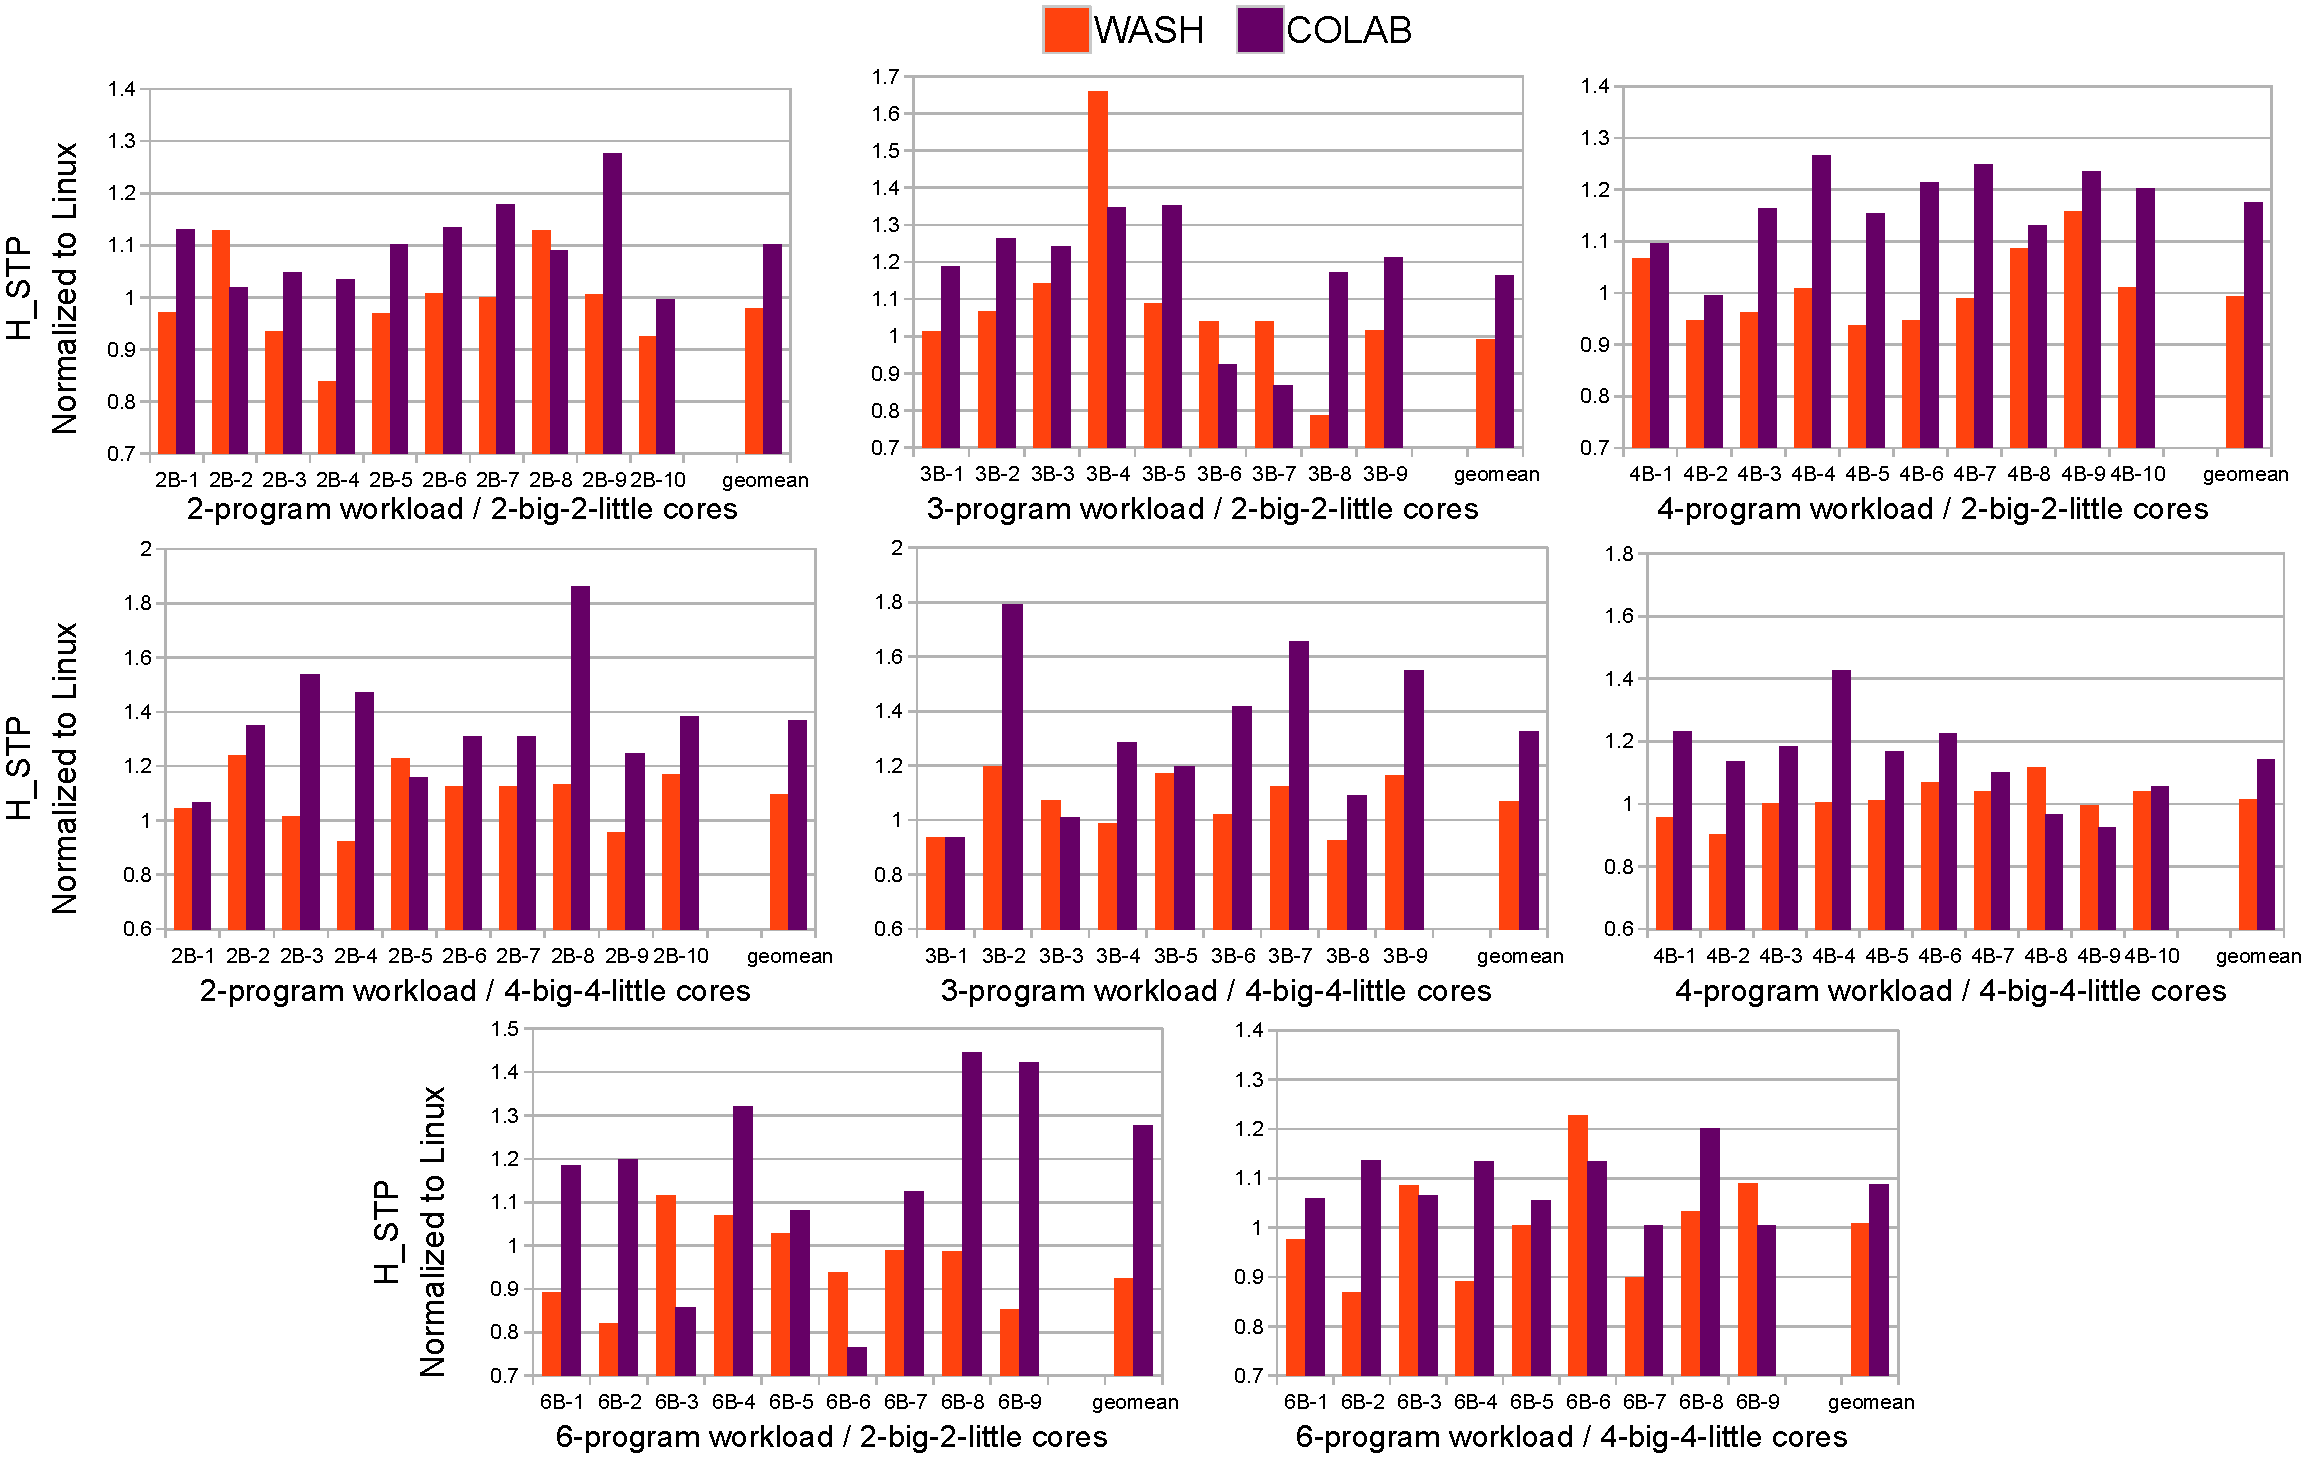
\includegraphics[scale=0.4]{figures/HSTP_NEW.pdf}
\caption{Heterogeneous System Throughput (H\_STP) of multiprogrammed workloads on 2-big-2-little and 4-big-4-little configurations. All results are normalized to the Linux CFS ones. Higher is better.}
\label{M36W}
\end{figure*} 
\textbf{\textit{Heterogeneous System Throughput:}}
Figure~\ref{M36W} shows our results for Heterogeneous System Throughput (H\_STP). As in the previous subsection, each subplot contains data for one hardware configuration and a specific number of co-scheduled programs.

Linux CFS and WASH do slightly better than COLAB in a few cases as our policy targets turnaround time optimization and will make decisions that hurt throughput in order to maintain some fairness. Still, on average our approach does better than CFS and WASH for most configurations. For certain asymmetric multi-program workloads, COLAB achieves not only acceptable throughput but significant improvement over its competition. By distributing bottleneck threads more evenly across cores, it makes better use of the system resources, avoiding leaving cores idle. This translates into up to 86\% higher throughput performance gain on the 4-big-4-little system, for 2B-8, and up-to 44\% higher throughput on the 2-big-2-little system, for 6B-8.
%Towards all 76 individual cases, other approaches only better than us on 3 cases and our approach only less than 10\% worse than them in the worst case (3B-6 on the 2-big-2-little configuration). 
%The collaboration-only approach can also do better than both Linux and WASH in most cases but worse than our final approach equipped with the multi-factor Coordinated model.

%with up-to 34\% improvement of H\_STP against other approaches. It does at most 15\% worse than WASH in the worst case (2B-2). Linux can also do slightly better than both WASH and our approach for some workloads (2B-10). As for the geomean of the multiple tests, our approach results in around 5\% performance gain of H\_ANTT against Linux CFS, while both WASH and the collaboration-only approach can not do better than Linux. The collaboration-only approach can achieve around 5\% improvement of H\_STP against Linux and WASH, and the improvement grows up to more than 10\% by applying our final approach. 

%The results on 4-benchmark workloads are shown in the lower two graphs of figure \ref{M24W}.Our approach can achieve up-to 39\% performance gain of H\_ANTT on certain workloads (4B-7) and up-to 40\% improvement of H\_STP on (4B-7). It does at most 10\% worse than WASH in the worst case (4B-9). Linux can also do better than both WASH and our approach for some workloads (4B-9). As for the geomean of the multiple tests, both the collaboration-only and our final approach results in around 9\% performance gain of H\_ANTT against WASH and 7\% against Linux. The collaboration-only approach can achieve around 14\% improvement of H\_STP against Linux and WASH, and the improvement grows up to more than 19\% by applying our final approach.  

%\textbf{\textit{Multi/single-thread Multi-program Workloads}}
 
%The results on 3-benchmark workloads are shown in the upper two graphs of figure \ref{M36W}.
%Our approach can achieve up-to 54\% performance gain of H\_ANTT on certain workloads (3B-2) and up-to 33\% improvement of H\_STP on (3B-1). It can always keep better than WASH in the all workload cases. Linux can also do slightly better than both WASH and our approach for some workloads (3B-6). As for the geomean of the multiple tests, the collaboration-only approach obtains around 5\% performance gain of H\_ANTT against Linux and WASH is not better than Linux. Our final approach can achieve 20\% performance gain against Linux and 25\% against WASH. The collaboration-only approach can achieve around 13\% improvement of H\_STP against Linux and WASH, and the improvement grows up to more than 18\% by applying our final approach.  
 
%The results on 6-benchmark workloads are shown in the lower two graphs of figure \ref{M36W}.
%Our approach can achieve up-to 54\% performance gain of H\_ANTT on certain workloads (6B-3) and up-to 46\% improvement of H\_STP on (6B-4). Linux can also do slightly better than both WASH and our approach for some workloads (6B-1,6B-5). As for the geomean of the multiple tests, the collaboration-only approach obtains around 17\% performance gain of H\_ANTT against Linux and WASH is not better than Linux. Our final approach can achieve 23\% performance gain against Linux and 27\% against WASH. The collaboration-only approach can achieve around 16\% improvement of H\_STP against Linux and WASH, and the improvement grows up to more than 20\% by applying our final approach.  



\textbf{\textit{Experimental Summary}} As shown in the results, the state-of-the-art AMP-aware WASH scheduler struggles to make good decisions as the number of co-scheduled programs rises. Trying to handle both core sensitivity and bottleneck acceleration through thread affinity alone may lead to too many threads assigned to big cores. Instead, we handle the two optimization aims separately. We assign on big cores only threads which run significantly faster on them and we prioritize running bottleneck threads regardless of their thread affinity. This leads to improved turnaround time, higher throughput, and better use of the processor resources compared to both CFS and WASH.
%\vspace{10mm}
\section{Conclusion}
This paper presents a novel scheduling framework targeting multi-threaded multiprogrammed workloads on asymmetric multicore processors. This scheduler is the first to account for all three factors affecting AMP scheduling: core affinity, thread criticality, and scheduling fairness, using a general purpose asymmetry-aware scheduler.

Over a representative selection of multi-programmed workloads, 
%we achieve more than 10\% performance gain compared to Linux, and more than 5\% performance gain to a state-of-the-art heterogeneous-aware scheduler on average.
Our COLAB improves performance by up to 25\% and 21\% lower trunaround time, 11\% and 5\% on average with similar advantage on throughput, compared to Linux and a state-of-the-art heterogeneity-aware scheduler.

%27\% on average on different hardware setups when compared to the Linux CFS scheduler and

%Compared with the default Linux CFS scheduler and the state-of-the-art AMP-aware WASH scheduler, COLAB achieves up-to 51\% performance gain in heterogeneous average normalized turnaround time (H\_ANTT) while 5\% to 27\% on average depending on the hardware setup and up-to 30\% increase on heterogeneous system throughput (H\_STP) in geomean targeting multi-threaded multiprogrammed co-executed workloads. 
%It performs significantly better when workloads contain both multi-threaded and single-thread applications achieving performance gain up to 54\% in average normalized turnaround time and 46\% increase on system throughput against both the previous approaches.

%COLAB aims to highlight the potential of further performance gain for AMP-aware scheduler targeting multi-threaded multiprogrammed co-execution and encourage following research by applying coordinated multi-factor runtime frameworks with core allocator and thread selector collaboration. 

%% Acknowledgments
%\section*{acks}
% List grants

%%%%%%%%% -- BIB STYLE AND FILE -- %%%%%%%%
\bibliographystyle{ieeetr}
\bibliography{references}
%%%%%%%%%%%%%%%%%%%%%%%%%%%%%%%%%%%%

\end{document}
